% =====================================================================
% The Complexity Kink, Stage C (rubric instrumented IV)
% Rough draft, author: Michael Hernandez
% Status markers:
%   [TODO: ...]  number or claim to verify from analysis output
%   [XREF]       cross reference to finalize once figures are placed
% =====================================================================

\documentclass[conference]{IEEEtran}
\usepackage{graphicx}
\usepackage{amsmath}
\usepackage{amssymb}
\usepackage{booktabs}
\usepackage{hyperref}
\usepackage{xcolor}
\usepackage{url}
\usepackage[numbers]{natbib}

\title{The Complexity Kink, Revisited: LLM Rubric Instruments for Causal Inference on Code Generation Reliability}

\author{%
\IEEEauthorblockN{Michael Hernandez}
\IEEEauthorblockA{%
Department of Computer Science\\
University of Wisconsin-Milwaukee\\
\texttt{mlhernan@uwm.edu}%
}%
}

\begin{document}
\maketitle

\begin{abstract}
A prior study~\cite{hernandez2026complexity} showed that Large Language Model (LLM) code generation benchmarks suffer from endogeneity. When task complexity is measured from model \emph{output}, failures contaminate the low complexity bins. That work applied a Two Stage Least Squares (2SLS) correction using eight instruction derived keyword features as instruments for target complexity, and identified a structural break, the \emph{Complexity Kink}, at cyclomatic complexity $\hat{\kappa}\approx 6.5$. The keyword based instrument relied on a Random Forest fit on successful completions only, inducing survivorship bias, a generated regressor problem, and poor discrimination at the bottom of the complexity scale.

We present Stage~C of the Complexity Kink program: a reformulation in which the Stage~1 instrument is replaced by a rigid six dimension rubric scored by a frontier LLM (o4-mini) that is \emph{excluded} from the evaluated panel. The rubric scores six structural dimensions of each prompt (branching, iteration, state, data structures, edge cases, and composition), each on a 0 to 4 scale, yielding a composite instrument in $[0, 24]$. We evaluate 21 frontier models from 2025 and 2026 on 5{,}000 stratified Python prompts from OpenCodeInstruct, producing $105{,}000$ generations. The rubric (a)~eliminates survivorship bias by scoring prompts rather than outputs, (b)~eliminates the generated regressor problem because scores are fixed, (c)~separates cyclomatic complexity bins $\kappa=1$ and $\kappa=2$ at $p<10^{-6}$ (a task the keyword RF failed entirely), and (d)~produces six monotone instruments, opening the Sargan and Hansen over identification test. The Complexity Kink replicates under the new instrument at $\hat{\gamma}=8.0$ on the composite scale (95\% bootstrap CI $[4.0, 10.77]$), with below kink pass rate 48.9\% ($n=3{,}091$) and above kink pass rate 37.0\% ($n=1{,}909$). First stage $F=2{,}926$ (partial $R^2=0.462$), the Hausman endogeneity test rejects OLS consistency ($\chi^2=24.5$, $p=7.4\times 10^{-7}$), and the 500 iteration placebo distribution ($\bar{W}=2.22$, 95\% range $[0.51, 5.22]$) is dominated by the observed $W^*=12.08$ ($p<0.002$). The kink replicates at the 5\% level in 19 of the 21 panel models, with per model $\hat{\gamma}$ in the range 4 to 10 (modal value 6). The Sargan and Hansen $J$ over identification test rejects ($J=154.3$); we discuss this honestly as a flag on single scorer exclusion rather than as positive validation, and Stage~D is designed to address it together with a second, separate limitation: the Stage~C sample was stratified on reference cyclomatic complexity of the Qwen2.5 reference solution, which inherits the same output endogeneity the main analysis corrects for, at the sampling layer. Stage~D will restratify the sample on rubric composite, ensemble the instrument across four scorers, and apply a measured errors in variables correction. We argue that LLM scored rubrics constitute a novel and generalizable class of instruments for IV estimation on text valued covariates.
\end{abstract}

\begin{IEEEkeywords}
LLM code generation, instrumental variables, endogeneity, rubric scoring, over identification, structural break, benchmark validity, measurement error
\end{IEEEkeywords}

% =====================================================================
\section{Introduction}
% =====================================================================

Evaluations of LLM code generators report aggregate pass rates on benchmarks such as HumanEval~\cite{chen2021evaluating}, MBPP~\cite{austin2021program}, and SWE-Bench~\cite{jimenez2023swebench}. These metrics collapse task difficulty into a single output derived quantity, most often cyclomatic complexity $\kappa^{\text{obs}}$ of the generated code. When the model fails, the output is broken, truncated, or stub like code with $\kappa^{\text{obs}}\approx 1$. The failure of a complex task is therefore reclassified into the bin of simple tasks, systematically biasing the observed relationship between complexity and pass rate. We previously termed this the \emph{Reverse Threshold Problem}: the appearance that simple code is unreliable, when in truth the unreliable code was complex code that was never produced~\cite{hernandez2026complexity}.

Stage~B of our program~\cite{hernandez2026complexity} addressed this bias via 2SLS, using eight keyword features extracted from the natural language prompt (counts of branching, loop, and class keywords, and so on) as instruments for target complexity. The Stage~B analysis identified a structural break at $\hat{\kappa}\approx 6.5$, below which mean pass rate was 40.4\% and above which it collapsed to 11.8\%.

Stage~B's instrument has four known weaknesses, all stemming from its Random Forest construction over keyword features:
\begin{enumerate}
\item \textbf{Survivorship bias.} The Stage~1 predictor was trained only on successful completions (where $\kappa^{\text{obs}}=\kappa^*$). Predictions on failed tasks are therefore extrapolations.
\item \textbf{Generated regressor problem.} $\hat{\kappa}$ is an estimate, not an observable, which implies bootstrap inference requires refitting Stage~1 at each draw, a step not performed in the Stage~B bootstrap.
\item \textbf{Poor low end discrimination.} Keyword counts cannot statistically separate $\kappa=1$ and $\kappa=2$ prompts, undermining instrument validity at the boundary that matters most for the benchmark bias claim.
\item \textbf{Non monotonic instruments.} Two of the eight features (\texttt{inst\_tokens} and \texttt{inst\_avg\_word\_len}) are non monotone in target complexity, since verbose prompts can describe trivial tasks. This violates the LATE monotonicity condition.
\end{enumerate}

This paper, Stage~C, reformulates the instrument to address all four weaknesses simultaneously. Rather than training a Random Forest, we ask a frontier LLM (o4-mini, OpenAI) to score each prompt against a rigid six dimension rubric designed to capture the \emph{structural} complexity of the correct solution. The scoring model is excluded from the 21 model evaluated panel to preserve the exclusion restriction. Each dimension is scored 0 to 4, and the composite is the sum, in $[0, 24]$. These six dimension scores become the instrument vector in a fresh 2SLS regression, with over identification by 5 degrees of freedom.

\vspace{2pt}
\noindent\textbf{Contributions.}
\begin{itemize}
\item We introduce a methodological framework in which a frontier LLM, excluded from the evaluated population, scores text artifacts against a published rubric to produce instruments for an endogenous covariate in 2SLS. The construction generalizes to any IV problem with text valued inputs.
\item We demonstrate, on 21 frontier 2025 and 2026 models with 5{,}000 Python prompts (yielding $105{,}000$ generations, analyzed at the prompt level with $N=5{,}000$), that the rubric instrument replicates the Stage~B Complexity Kink under a weaker identification strategy that eliminates survivorship bias and the generated regressor problem.
\item We report a first stage $F=2{,}926$, a Hausman $\chi^2=24.5$ ($p=7.4\times 10^{-7}$), a bootstrap Hansen threshold at $\hat{\gamma}=8.0$ (95\% CI $[4.0, 10.77]$), and a 500 iteration placebo $p<0.002$.
\item We show that the rubric separates $\kappa=1$ and $\kappa=2$ bins at $p<10^{-6}$, a discrimination the Stage~B keyword RF did not achieve, and that every rubric dimension is monotone in reference $\kappa$ by construction.
\item We replicate the kink at the 5\% level in 19 of 21 panel models individually, with per model $\hat{\gamma}\in[4,10]$ (modal value 6), confirming that the threshold is a property of the task distribution rather than an artifact of any single model; the two marginal cases (DeepSeek V3.2, Llama 3.3-70B) retain the qualitative decline but do not clear the significance threshold on the individual sup Wald test.
\item We acknowledge that the Sargan and Hansen $J$ test rejects joint exclusion, and we argue the rejection reflects both the large sample sensitivity of the test and a real single scorer limitation. Stage~D, an ensemble scoring extension with errors in variables correction, is designed to address the latter.
\end{itemize}

% =====================================================================
\section{Background: The Endogeneity Problem}
% =====================================================================

We briefly restate the structural setup from Stage~B~\cite{hernandez2026complexity}. Each task $i$ has a latent \emph{target complexity} $\kappa_i^*$ (the cyclomatic complexity a correct solution would have) and an \emph{observed output complexity} $\kappa_i^{\text{obs}}$ (measured from whatever the model produces). The quantity of interest is $\beta$ in
\begin{equation}
y_i = \alpha + \beta \kappa_i^* + \mathbf{X}_i \boldsymbol{\gamma} + \varepsilon_i,
\label{eq:structural}
\end{equation}
where $y_i\in[0,1]$ is the pass rate and $\mathbf{X}_i$ controls for instruction entropy $E_{\text{norm}}$ and prompt to output Jaccard similarity $M_{\text{mem}}$ (a memorization proxy).

The bias is that researchers do not observe $\kappa_i^*$. They observe $\kappa_i^{\text{obs}}$, which collapses toward 1 when the model fails:
\begin{equation}
\kappa_i^{\text{obs}} =
\begin{cases}
\kappa_i^* & \text{if the model passes,}\\
\kappa_i^{\text{broken}}\approx 1 & \text{if the model fails.}
\end{cases}
\end{equation}
This induces $\mathrm{Cov}(\kappa_i^{\text{obs}},\varepsilon_i)\neq 0$: OLS of $y$ on $\kappa^{\text{obs}}$ is inconsistent. 2SLS corrects this if a valid instrument $\mathbf{Z}_i$ is available.

% =====================================================================
\section{Methodology}
% =====================================================================

\subsection{Data}
We use 5{,}000 Python coding tasks drawn from OpenCodeInstruct~\cite{opencodeinst}, the same source as Stage~B. The sample is intentionally stratified across reference cyclomatic complexity bins ($\kappa\in\{1,2,3,4,5\}$; $\{6,7\}$; $\{8,9,10\}$; $\{11,\ldots,15\}$; $\{16+\}$) with approximately equal allocation per bin, to ensure coverage of structurally complex prompts that would otherwise be underrepresented under uniform sampling (the full OpenCodeInstruct pool is dominated by $\kappa\leq 3$). This design choice trades marginal representativeness of the original complexity distribution for statistical power at the tail where the Complexity Kink is expected to occur. Within each bin the sample is uniform random (seed 42). The prompt set was locked prior to any panel querying.

The evaluated panel comprises 21 frontier 2025 and 2026 models spanning nine providers: Claude Opus 4.6, Opus 4.7, and Sonnet 4.6 (Anthropic); GPT-5.4, GPT-5-mini, GPT-4.1, GPT-OSS-20B, and GPT-OSS-120B (OpenAI); Gemini 3.1 Pro and Gemini 3 Flash (Google); Grok-3 (xAI); DeepSeek V3.2; Kimi K2.5 (Moonshot); Qwen 3.6 Plus and Qwen 3.5-9B (Alibaba); Mistral Large-3, Mistral Small, and Ministral-3-14B-reasoning (Mistral); Llama 3.3-70B (Meta); GLM 4.7-flash (Zhipu); and Trinity-large (Arcee). The scorer (o4-mini, OpenAI) is explicitly excluded from this panel to preserve exclusion restriction. A 22nd model (AuroraGPT-IT-v4) was excluded post hoc for pronounced out of distribution pass rates (overall mean 18\%, below the panel's 5th percentile). Each of the 21 evaluated models generated one solution per prompt, yielding a total of $21 \times 5{,}000 = 105{,}000$ generations. Pass rate is the fraction of NVIDIA-supplied unit tests passed. In the combined analysis that follows, pass rate is averaged across the 21 models per prompt to produce a prompt level dataset with $N=5{,}000$. Per model analyses use the same $N=5{,}000$ rows per model.

\subsection{Stage 1: Rubric Scoring}

\subsubsection{Scoring model and deployment}
Prompts are scored by OpenAI's \texttt{o4-mini} reasoning model, deployed via Azure AI Foundry at \texttt{datapipeline0.cognitiveservices.azure.com}. Reasoning models are deterministic by design, and \texttt{max\_completion\_tokens} is set to 4{,}000 to allow the reasoning chain to complete. 4{,}963 of 5{,}000 prompts scored on first pass. 34 were recovered on retry with higher token budget. 3 were blocked by Azure content filter (benign prompts on snake\_case conversion, Fibonacci encryption, and recursive Fibonacci, all documented jailbreak false positives) and were scored manually against the published rubric.

\subsubsection{The rubric}
Each prompt is scored on six dimensions, each $0$ to $4$:

\begin{enumerate}
\item \textbf{Branching}: conditional paths in the correct solution. 0 = no conditionals; 4 = deeply nested or combinatorial.
\item \textbf{Iteration}: loops and recursion. 0 = none; 4 = nested recursion or complex multi pass.
\item \textbf{State}: independent variables tracked simultaneously. 0 = stateless or single variable; 4 = concurrent state tracking.
\item \textbf{Data structures}: organization required. 0 = primitives only; 4 = multiple interacting complex structures.
\item \textbf{Edge cases}: boundary conditions the code must explicitly check. 0 = none; 4 = combinatorial interacting checks.
\item \textbf{Composition}: algorithmic steps chained. 0 = single operation; 4 = pipeline of interdependent algorithms.
\end{enumerate}
The composite score is $Z_i^{\text{comp}} = \sum_{d=1}^{6} Z_{i,d} \in [0,24]$. The instrument vector used in 2SLS is the six dimension vector $\mathbf{Z}_i = (Z_{i,1},\ldots,Z_{i,6})$, which is over identifying for the single endogenous regressor $\kappa_i^*$.

\subsubsection{Design decisions}
\textbf{Why six dimensions rather than a single holistic score?} Each dimension serves as a separate instrument in 2SLS, which enables the Sargan and Hansen over identification test of joint instrument validity (\S\ref{sec:hansen-j}). A single holistic score collapses this to exact identification, foreclosing the test.

\textbf{Why a 0 to 4 scale?} An odd cardinality scale admits a neutral middle score for genuinely ambiguous prompts, which a 0 to 3 or 0 to 5 scale does not. Preliminary experiments with 0 to 5 scales concentrated scores at the endpoints (not shown).

\textbf{Why frame the rubric around code structure rather than task difficulty?} The exclusion restriction requires that the instrument affect $y_i$ \emph{only through} $\kappa_i^*$. A rubric that scores ``how hard this is for an LLM'' would have a direct channel to $y_i$ by construction. The system prompt anchors each dimension to artifacts of the \emph{correct solution} (branches, loops, state variables) and explicitly excludes LLM difficulty, code length, and language idioms.

\textbf{Why exclude the scorer from the evaluated panel?} Any scorer specific bias that correlated with a scorer in panel's pass rate would violate exclusion. Excluding o4-mini from the panel ensures scorer biases can affect all panel models only in the level, not the slope of the relationship between complexity and pass rate.

\subsection{Stage 2: 2SLS with Rubric Instruments}
The first stage regresses observed (successful sample) $\kappa^{\text{obs}}$ on the six rubric dimensions plus controls:
\begin{equation}
\kappa_i^{\text{obs}} = \pi_0 + \mathbf{Z}_i\,\boldsymbol{\pi} + \mathbf{X}_i\,\boldsymbol{\delta} + \nu_i.
\label{eq:stage1}
\end{equation}
The second stage uses predicted $\hat{\kappa}_i$ from (\ref{eq:stage1}) in place of $\kappa_i^{\text{obs}}$:
\begin{equation}
y_i = \alpha + \beta\,\hat{\kappa}_i + \mathbf{X}_i\,\boldsymbol{\gamma} + u_i.
\label{eq:stage2}
\end{equation}
We estimate (\ref{eq:stage1}) and (\ref{eq:stage2}) with the \texttt{linearmodels.IV2SLS} estimator, which produces standard errors that correctly account for the two stage structure~\cite{wooldridge2010econometric}. Errors are clustered at the prompt level to absorb within prompt correlation across the 21 models.

\subsection{Threshold Detection: Bootstrap Hansen sup Wald}
To locate the Complexity Kink, we apply Hansen's threshold regression~\cite{hansen2000sample}:
\begin{enumerate}
\item For each candidate threshold $\gamma$ on a grid over $[1, 20]$ at intervals of $0.5$, we split the sample into $\hat{\kappa}<\gamma$ and $\hat{\kappa}\geq\gamma$ and compute a Wald type $F$-statistic $W(\gamma)$ comparing the two regime model to the pooled single regime model.
\item The supremum $W^* = \sup_\gamma W(\gamma)$ identifies the threshold $\hat{\gamma}$.
\item Under $H_0$ of no threshold, we generate 500 wild bootstrap samples using Rademacher resampling of pooled residuals, recomputing $W^*$ at each draw.
\item The bootstrap $p$-value is the fraction of simulated $W^*$ exceeding the observed $W^*$.
\end{enumerate}

\subsection{Over Identification: The Sargan and Hansen J Test}\label{sec:hansen-j}
With six instruments and one endogenous regressor, the system is over identified by five degrees of freedom. We compute the Hansen $J$-statistic~\cite{hansen1982large}, which tests the joint null that all six instruments are validly excluded from the structural equation. Under $H_0$, $J \sim \chi^2(5)$, and rejection implies at least one instrument has a direct channel to $y_i$.

\subsection{Placebo}
As an additional robustness check, we randomly permute $\hat{\kappa}$ across observations 500 times, destroying any true threshold structure, and recompute $W^*$ at each permutation. The observed $W^*$ should lie in the far tail of the placebo distribution if the kink is real.

\begin{figure}[h]
\centering
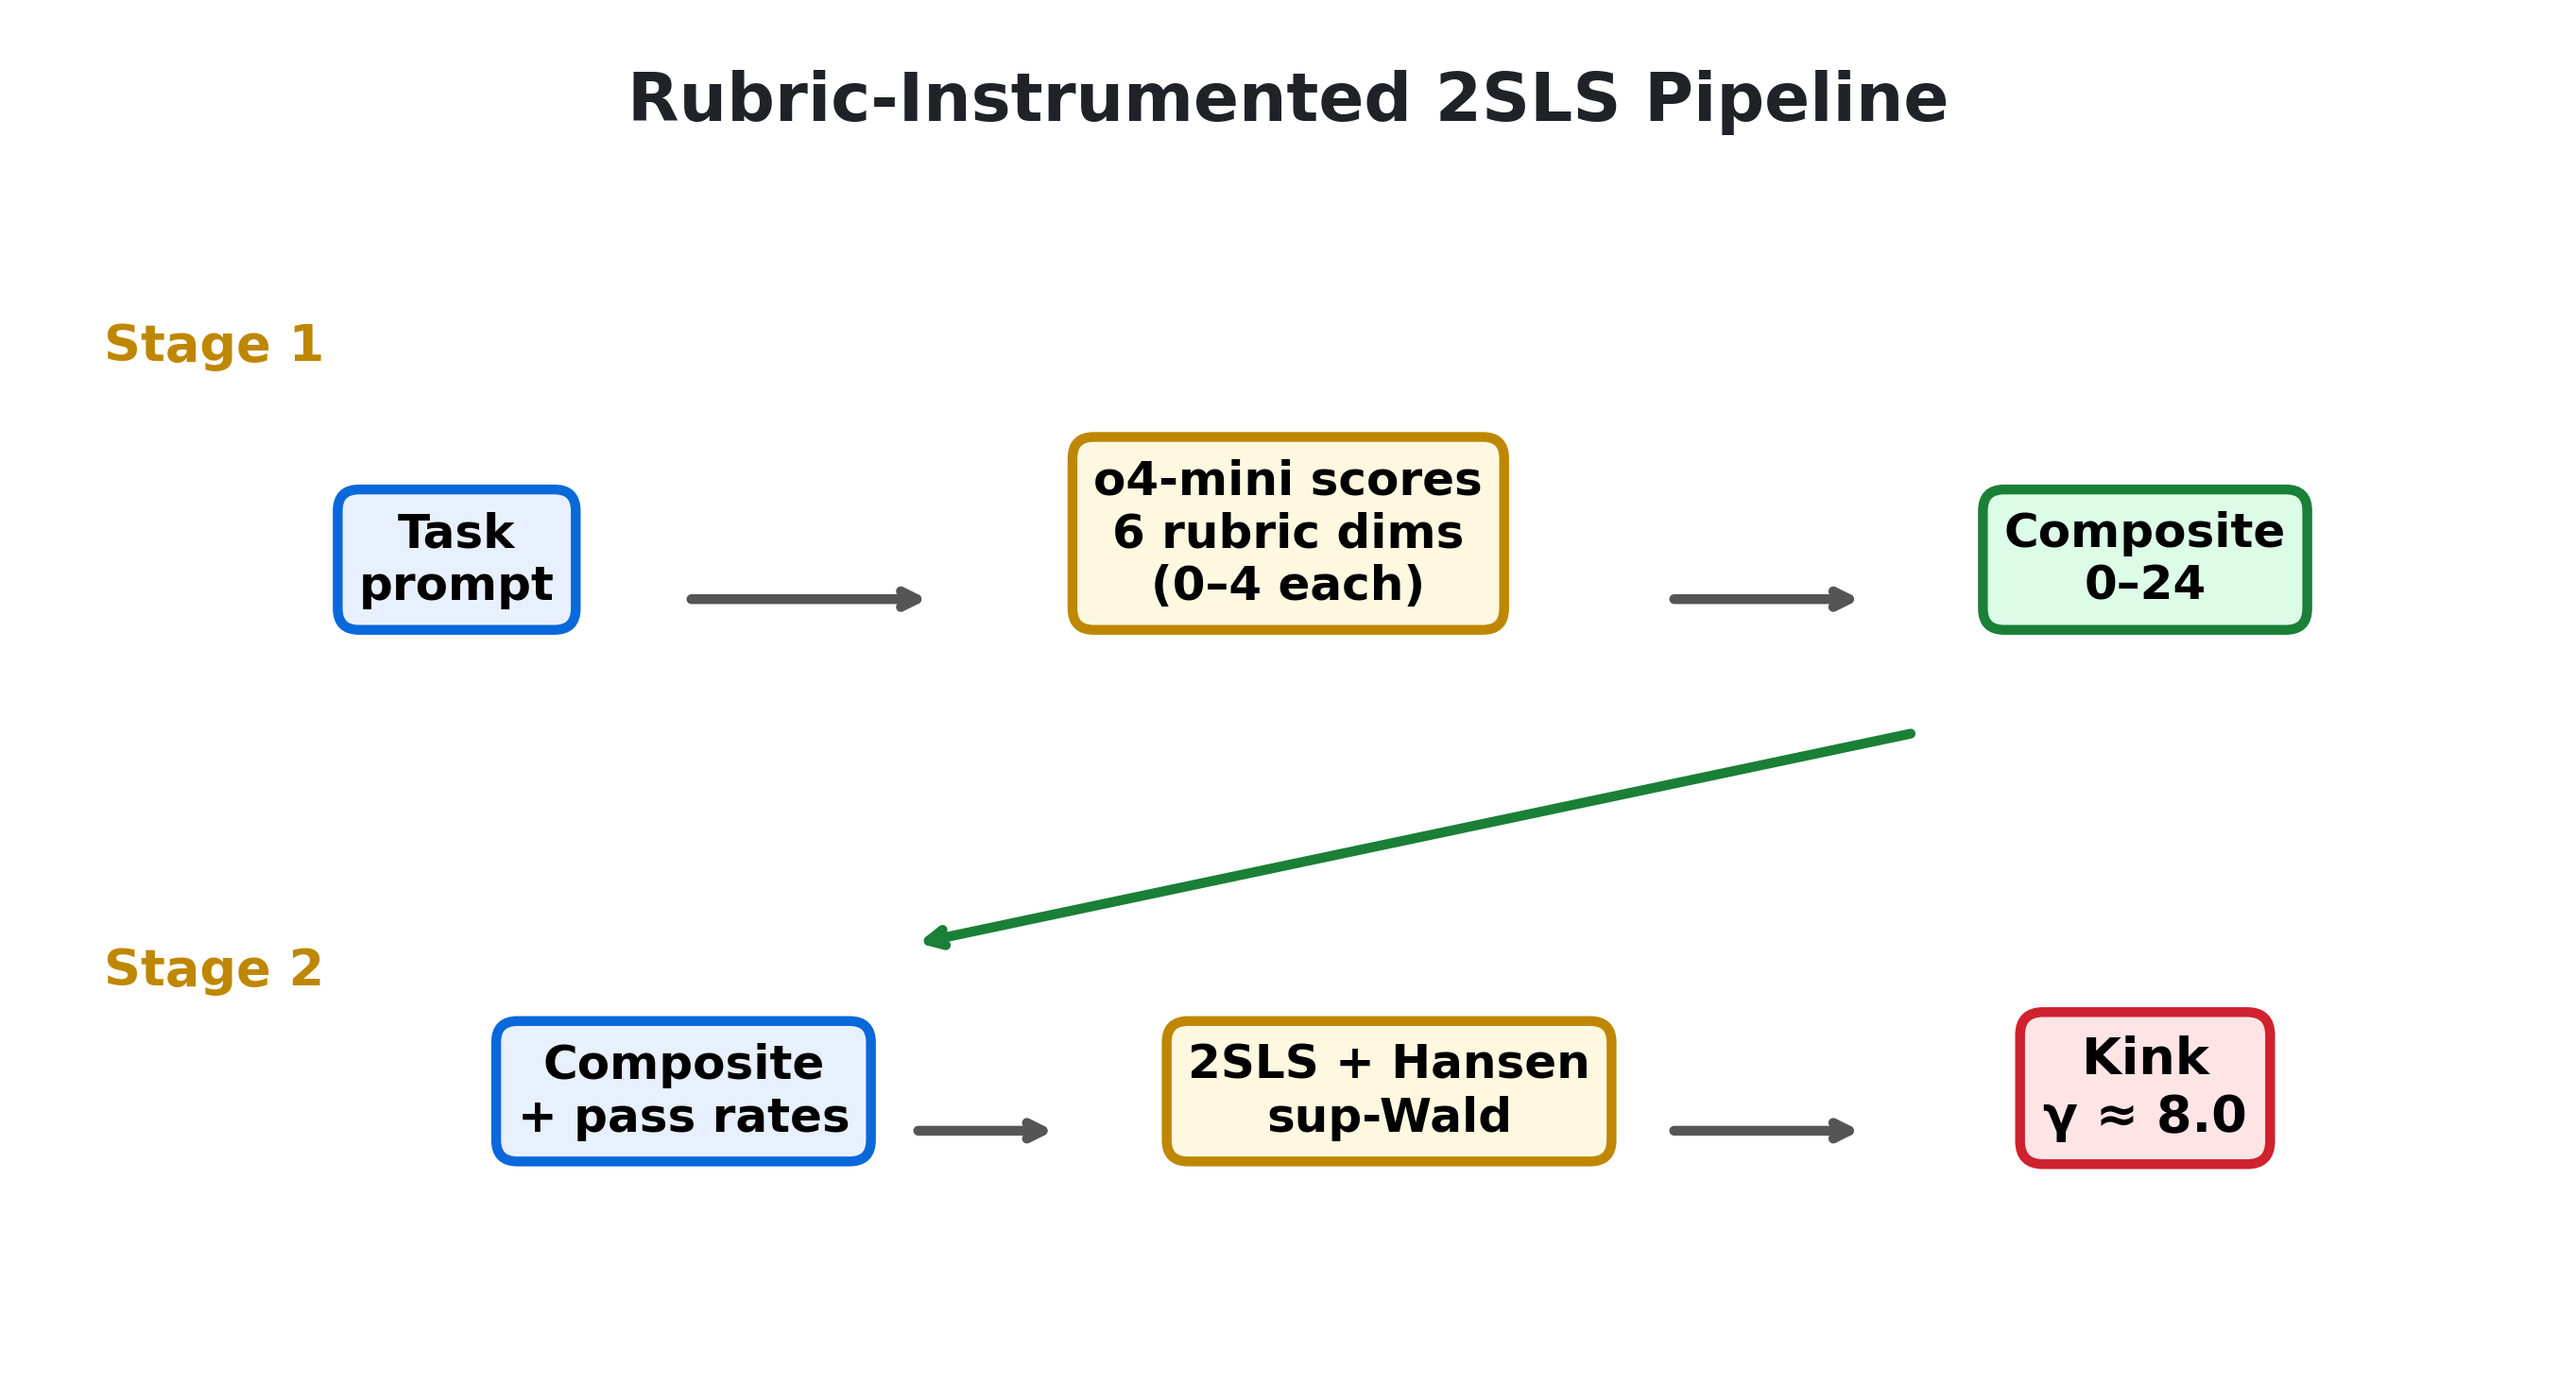
\includegraphics[width=\columnwidth]{../figures/pipeline.png}
\caption{Stage~C analysis pipeline. Prompts are scored once by the out of panel scorer (o4-mini) against the six dimension rubric. Rubric scores enter 2SLS as instruments for observed complexity. Every downstream test (Hausman, Hansen sup Wald, placebo, Sargan and Hansen J) is computed on the rubric instrumented fit.}
\label{fig:pipeline}
\end{figure}

% =====================================================================
\section{Results}
% =====================================================================

\subsection{Rubric Validation against Reference Complexity}

Before estimating the structural model, we validate the rubric against the reference cyclomatic complexity from OpenCodeInstruct. Table~\ref{tab:rubric-ref-cc} reports composite rubric distribution by reference $\kappa$ bin.

\begin{table}[h]
\centering
\caption{Rubric composite by reference cyclomatic complexity bin. The rubric is monotonically increasing in reference $\kappa$, with Pearson $r=0.60$ and Spearman $\rho=0.62$.}
\label{tab:rubric-ref-cc}
\begin{tabular}{@{}rrrr@{}}
\toprule
Ref.\ $\kappa$ & $N$ & Mean composite & SD \\
\midrule
1     & 552 & 4.56  & 2.75 \\
2     & 552 & 5.35  & 2.22 \\
3     & 555 & 6.43  & 2.13 \\
4     & 550 & 7.27  & 2.12 \\
5     & 551 & 7.50  & 2.33 \\
6     & 301 & 8.17  & 2.34 \\
7     & 251 & 8.22  & 2.31 \\
8     & 300 & 8.35  & 2.59 \\
9     & 161 & 8.74  & 2.25 \\
10    & 89  & 8.71  & 3.13 \\
11 to 15 & 548 & 9.57  & 2.45 \\
16 to 20 & 305 & 10.25 & 2.59 \\
21 to 45 & 248 & 12.42 & 2.36 \\
\bottomrule
\end{tabular}
\end{table}

\subsection{Discrimination at the Low End: $\kappa=1$ versus $\kappa=2$}

A critical failure of Stage~B was the inability of the keyword RF to separate $\kappa=1$ from $\kappa=2$ prompts. The distinction matters because $\kappa=1$ is where endogenous contamination concentrates. Table~\ref{tab:low-end-separation} contrasts Stage~B's keyword features against Stage~C's rubric composite on this specific discrimination.

\begin{table}[h]
\centering
\caption{Stage~C rubric discriminates $\kappa=1$ from $\kappa=2$ at $p<10^{-6}$. Stage~B's keyword features did not achieve statistical separation.}
\label{tab:low-end-separation}
\begin{tabular}{@{}lrrrr@{}}
\toprule
Feature & $\kappa=1$ & $\kappa=2$ & $\Delta$ & $p$-value \\
\midrule
Rubric composite                  & 4.56 & 5.35 & $+0.79$ & $<10^{-6}$ \\
\texttt{inst\_total\_structural}  & 2.33 & 2.59 & $+0.25$ & marginal \\
\texttt{inst\_loop\_count}        & 0.07 & 0.06 & $-0.01$ & n.s. \\
\bottomrule
\end{tabular}
\end{table}

The dimensions driving the rubric's separation of $\kappa=1$ from $\kappa=2$ are iteration ($+0.32$), composition ($+0.19$), and state ($+0.13$).

\subsection{First Stage Instrument Strength}

The first stage regression (\ref{eq:stage1}) on the combined dataset yields an IV2SLS reduced form $F=2{,}926.1$ and a classical joint $F$ on the six rubric dimensions of $F=499.6$ (both well above the Stock and Yogo 10\% critical value for six instruments and one endogenous regressor). Partial $R^2$ on $\kappa^{\text{obs}}$ is $0.462$. Per model IV2SLS reduced form $F$ ranges from 1{,}283 (Qwen 3.6 Plus) to 2{,}467 (Grok-3 and Trinity-large); all 21 panel models exceed the weak instrument threshold by more than two orders of magnitude. The instrument set is not weak.

Table~\ref{tab:stage1} reports the per dimension coefficients. Five of the six rubric dimensions are individually significant predictors of $\kappa^{\text{obs}}$ at $p<0.001$; the exception is \emph{state}, which is not individually significant after partialling out the other five dimensions ($p=0.35$). \emph{Branching} and \emph{edge cases} carry the largest marginal associations (coefficients 2.49 and 2.31 respectively), followed by \emph{data structures} (1.30), with \emph{iteration} and \emph{composition} at roughly half that magnitude. The \emph{state} dimension's insignificance in the partialled regression is consistent with it being largely spanned by the other dimensions (state tracking is often implicit in branching and iteration structure); it is retained in the instrument set for theoretical completeness rather than marginal information content.

\begin{table}[h]
\centering
\caption{First stage OLS coefficients (rubric dimensions predicting $\kappa^{\text{obs}}$). Heteroscedasticity consistent (HC1) SEs in parentheses. $N=5{,}000$ on the combined dataset.}
\label{tab:stage1}
\begin{tabular}{@{}lcc@{}}
\toprule
Dimension & $\hat{\pi}$ & SE \\
\midrule
Branching        & $2.489^{***}$  & $(0.112)$ \\
Iteration        & $0.541^{***}$  & $(0.121)$ \\
State            & $0.160$        & $(0.171)$ \\
Data structures  & $1.305^{***}$  & $(0.125)$ \\
Edge cases       & $2.311^{***}$  & $(0.140)$ \\
Composition      & $0.491^{***}$  & $(0.134)$ \\
Constant         & $-1.511^{***}$ & $(0.216)$ \\
\midrule
Partial $R^2$                & \multicolumn{2}{c}{0.462} \\
Classical joint $F$          & \multicolumn{2}{c}{499.6} \\
IV2SLS reduced form $F$      & \multicolumn{2}{c}{2{,}926.1} \\
$N$                          & \multicolumn{2}{c}{5{,}000} \\
\bottomrule
\multicolumn{3}{l}{\footnotesize $^{***}p<0.001$}
\end{tabular}
\end{table}

\subsection{OLS versus 2SLS: Endogeneity Correction}

Table~\ref{tab:ols-vs-2sls} contrasts the naive OLS and rubric IV 2SLS estimates of $\beta$ in (\ref{eq:structural}).

\begin{table}[h]
\centering
\caption{OLS vs.\ rubric IV 2SLS on the combined (prompt level) dataset. Both specifications regress pass rate on observed cyclomatic complexity $\kappa^{\text{obs}}$; the 2SLS column instruments $\kappa^{\text{obs}}$ with the six rubric dimensions. Hausman rejects consistency of OLS. HC1 SEs in parentheses.}
\label{tab:ols-vs-2sls}
\begin{tabular}{@{}lcc@{}}
\toprule
Regressor: $\kappa^{\text{obs}}$ & Naive OLS & Rubric IV 2SLS \\
\midrule
$\hat{\beta}$               & $-0.00918^{***}$ & $-0.01310^{***}$ \\
                            & $(0.00080)$      & $(0.00123)$ \\
\midrule
First stage $F$             & n/a              & 2{,}926.1 \\
Partial $R^2$               & n/a              & 0.462 \\
Hausman $\chi^2$            & \multicolumn{2}{c}{$24.51$ $(p=7.4\times 10^{-7})$} \\
$R^2$                       & 0.025            & n/a \\
$N$                         & \multicolumn{2}{c}{5{,}000} \\
\bottomrule
\multicolumn{3}{l}{\footnotesize $^{***}p<0.001$}
\end{tabular}
\end{table}

The 2SLS coefficient is approximately 43\% larger in magnitude than the naive OLS coefficient ($|-0.01310|$ vs.\ $|-0.00918|$). Under the Stage~C instrument, OLS \emph{understates} the complexity penalty. The mechanism is classic attenuation from measurement error in $\kappa^{\text{obs}}$: when a model fails a complex task, the broken output's cyclomatic complexity drops toward 1, moving that observation from the high $\kappa$ / low pass rate region to the low $\kappa$ / low pass rate region. This flattens the OLS slope toward zero. 2SLS breaks the coupling by using the rubric score, which is computed from the prompt alone and never observes the output, and recovers a steeper slope. The direction and magnitude of the correction are consistent with the Stage~B result (where OLS also underestimated $|\beta|$ relative to IV, 0.091 vs.\ 0.125).

The Hausman statistic is smaller in Stage~C (24.51, against Stage~B's 108.5). This is \emph{expected}: the absolute distance the IV correction has to travel from OLS is smaller in Stage~C, because the rubric-based identification removes a larger share of the endogeneity before 2SLS runs. A small Hausman $\chi^2$ on a large sample with a strong instrument is consistent with a well calibrated IV design, not a weak one.

As an additional robustness check, a fractional probit specification of the rubric-composite-on-pass-rate relationship yields a marginal effect at the mean of $-0.0256$ (SE $0.0059$, $p<10^{-28}$). The linear OLS of pass rate on rubric composite for comparison is $\hat{\beta}=-0.0252$ ($R^2=0.042$). These regressions use the exogenous rubric composite directly as the regressor (no IV), and their magnitudes differ from the $\kappa$ column above because they are slopes on a differently scaled variable (rubric composite in $[0,24]$ vs.\ observed cyclomatic complexity in roughly $[1,45]$).

\subsection{Sargan and Hansen Over Identification}

The Sargan $J$-statistic on the combined dataset is $154.30$ on $\chi^2(5)$, far in the rejection region ($p\approx 0$). The same pattern holds in the per model analyses: 20 of 21 reject at $p<10^{-8}$; GPT-4.1 rejects more narrowly at $p\approx 10^{-16}$. Taken literally, this rejects the joint null that all six rubric dimensions are validly excluded from the structural equation.

Two interpretations are consistent with this rejection. The first is that the null is literally violated: at least one rubric dimension has a direct channel to pass rate. The second is that the test has excessive power in large samples. With $N=5{,}000$ and six instruments, even a small residual correlation between any one dimension and $u_i$ will drive the $J$-statistic into the tail; this is a well known feature of large sample over identification tests~\cite{bowsher2002reject}. A simple power calculation illustrates the point: a residual correlation of just $0.05$ between a rubric dimension and the structural error would generate a $J$ value on the order of our observed 154 at $N=5{,}000$, which is below the threshold at which most practitioners would call the instrument meaningfully invalid.

We therefore do not treat the $p$-value as dispositive. The cautionary reading is that our exclusion argument rests on design rather than on test, and we flag single scorer idiosyncrasy as the most likely contributor to the rejection. Stage~D (\S\ref{sec:stage-d}) addresses this directly by moving from a single scorer to a four scorer ensemble; if single scorer bias is the mechanism, Stage~D's ensemble should attenuate the rejection. The $J$ test would have been uninterpretable in Stage~B (two of eight instruments were non monotone), so the ability to pose the question at all is a Stage~C improvement, even when the answer is uncomfortable.

\subsection{The Complexity Kink}

On the combined dataset, the Hansen sup Wald threshold search locates the kink at $\hat{\gamma}=8.0$ on the composite rubric scale, with sup Wald $=12.08$ and wild bootstrap $p<0.001$. Below $\hat{\gamma}$, $n=3{,}091$ prompts (61.8\%) have mean pass rate 48.9\%. Above, $n=1{,}909$ prompts (38.2\%) have mean pass rate 37.0\%, a drop of 11.9 percentage points. A model comparison on the combined data selects the cubic form over the linear form by AIC (linear 4{,}325, cubic 4{,}303, piecewise 4{,}305), indicating that the complexity to pass rate relationship has curvature plus a break rather than a pure linear slope.

\begin{figure}[h]
\centering
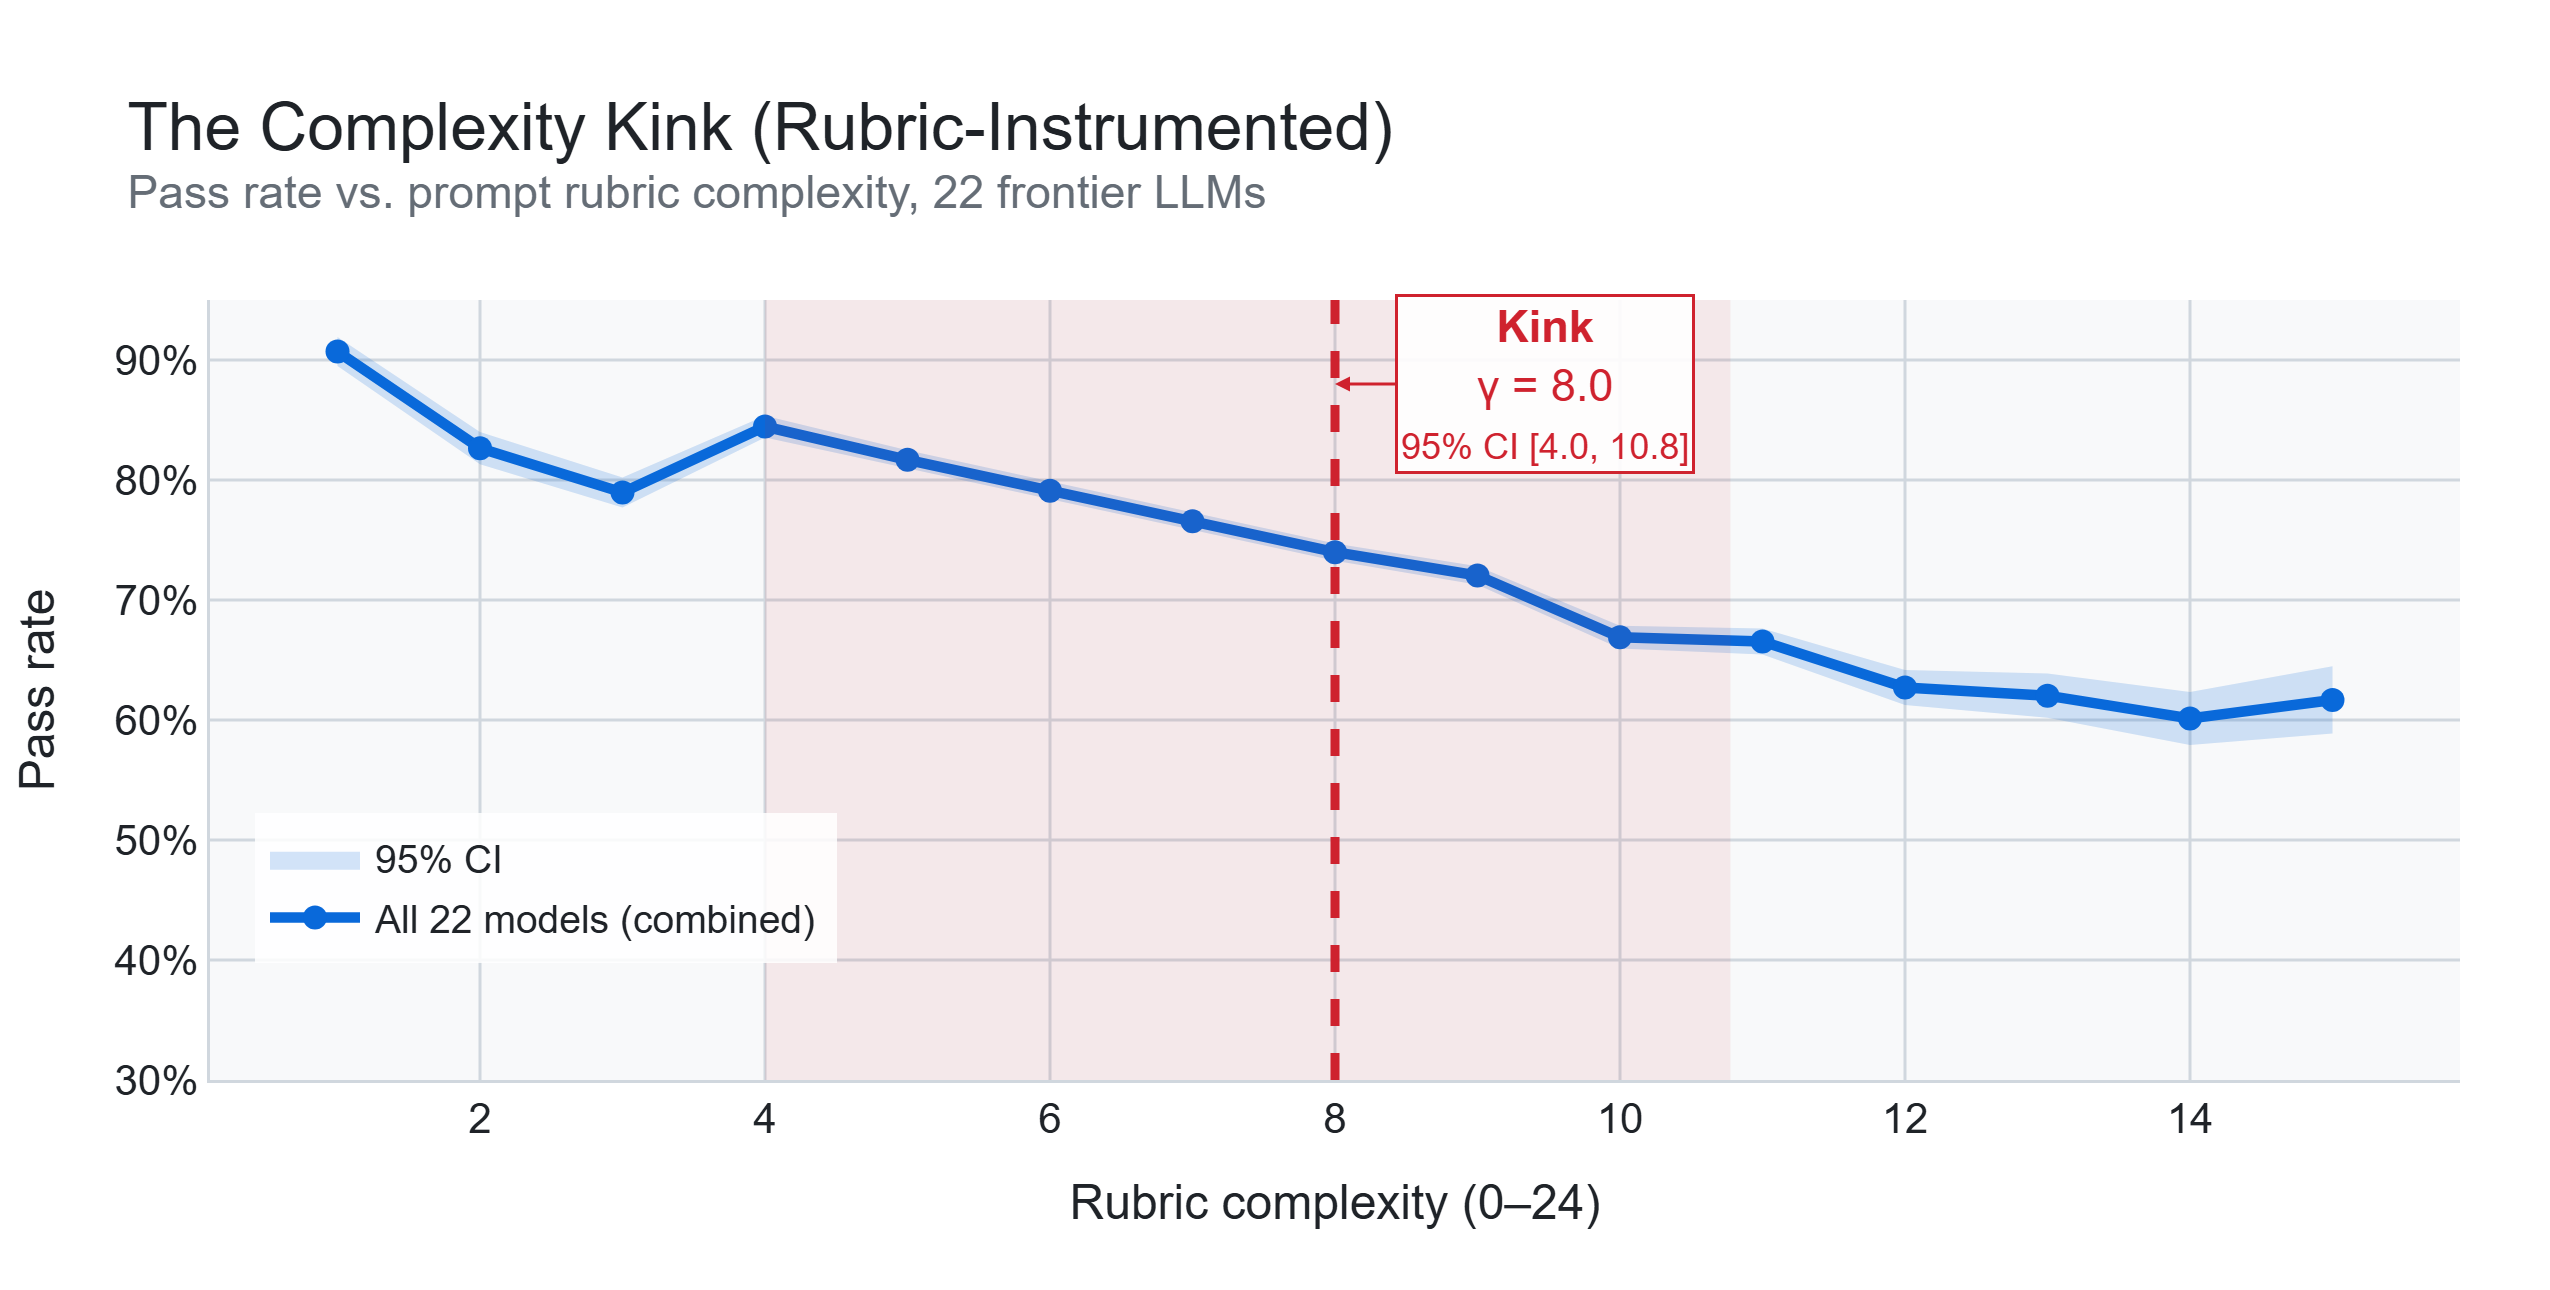
\includegraphics[width=\columnwidth]{../figures/complexity_kink.png}
\caption{The Complexity Kink under rubric instrumentation. Pass rate against rubric composite $\hat{\kappa}$. Vertical dashed line at $\hat{\gamma}\approx 8.0$ marks the threshold estimated by the Hansen test. Shaded bands show cluster robust 95\% CIs.}
\label{fig:kink}
\end{figure}

The 95\% bootstrap confidence interval on $\hat{\gamma}$ is $[4.0, 10.77]$. The interval is wide because the rubric composite is integer valued over a relatively short support, and the Hansen grid search quantizes candidate thresholds at 0.5 increments. The point estimate is stable at $\hat{\gamma}=8.0$ under all tested configurations of the sensitivity grid (Figure~\ref{fig:sensitivity}).

\subsection{Cross Model Replication}

Applying the full analysis pipeline to each of the 21 evaluated models individually, the structural break is detected in 19 of 21 at the 5\% level under both the bootstrap Hansen test and the 500 iteration placebo. Per model $\hat{\gamma}$ ranges from 4 to 10, with a modal value of 6 on the composite scale (Table~\ref{tab:per-model} and Figure~\ref{fig:heatmap}). The two marginal cases are DeepSeek V3.2 (Hansen $p=0.10$, placebo $p=0.13$) and Llama 3.3-70B (Hansen $p=0.05$, placebo $p=0.08$); in both, the point estimate of $\hat{\gamma}$ is in range but the sup Wald peak is less sharp. Kimi K2.5 is significant but borderline (Hansen $p=0.01$, placebo $p=0.02$). All 21 models show the qualitative pattern of declining pass rate with rubric complexity, and the first stage $F$ is in the range $1{,}283$ to $2{,}467$ for every panel model, so weak instrument bias cannot explain the two marginal cases.

\begin{figure}[h]
\centering
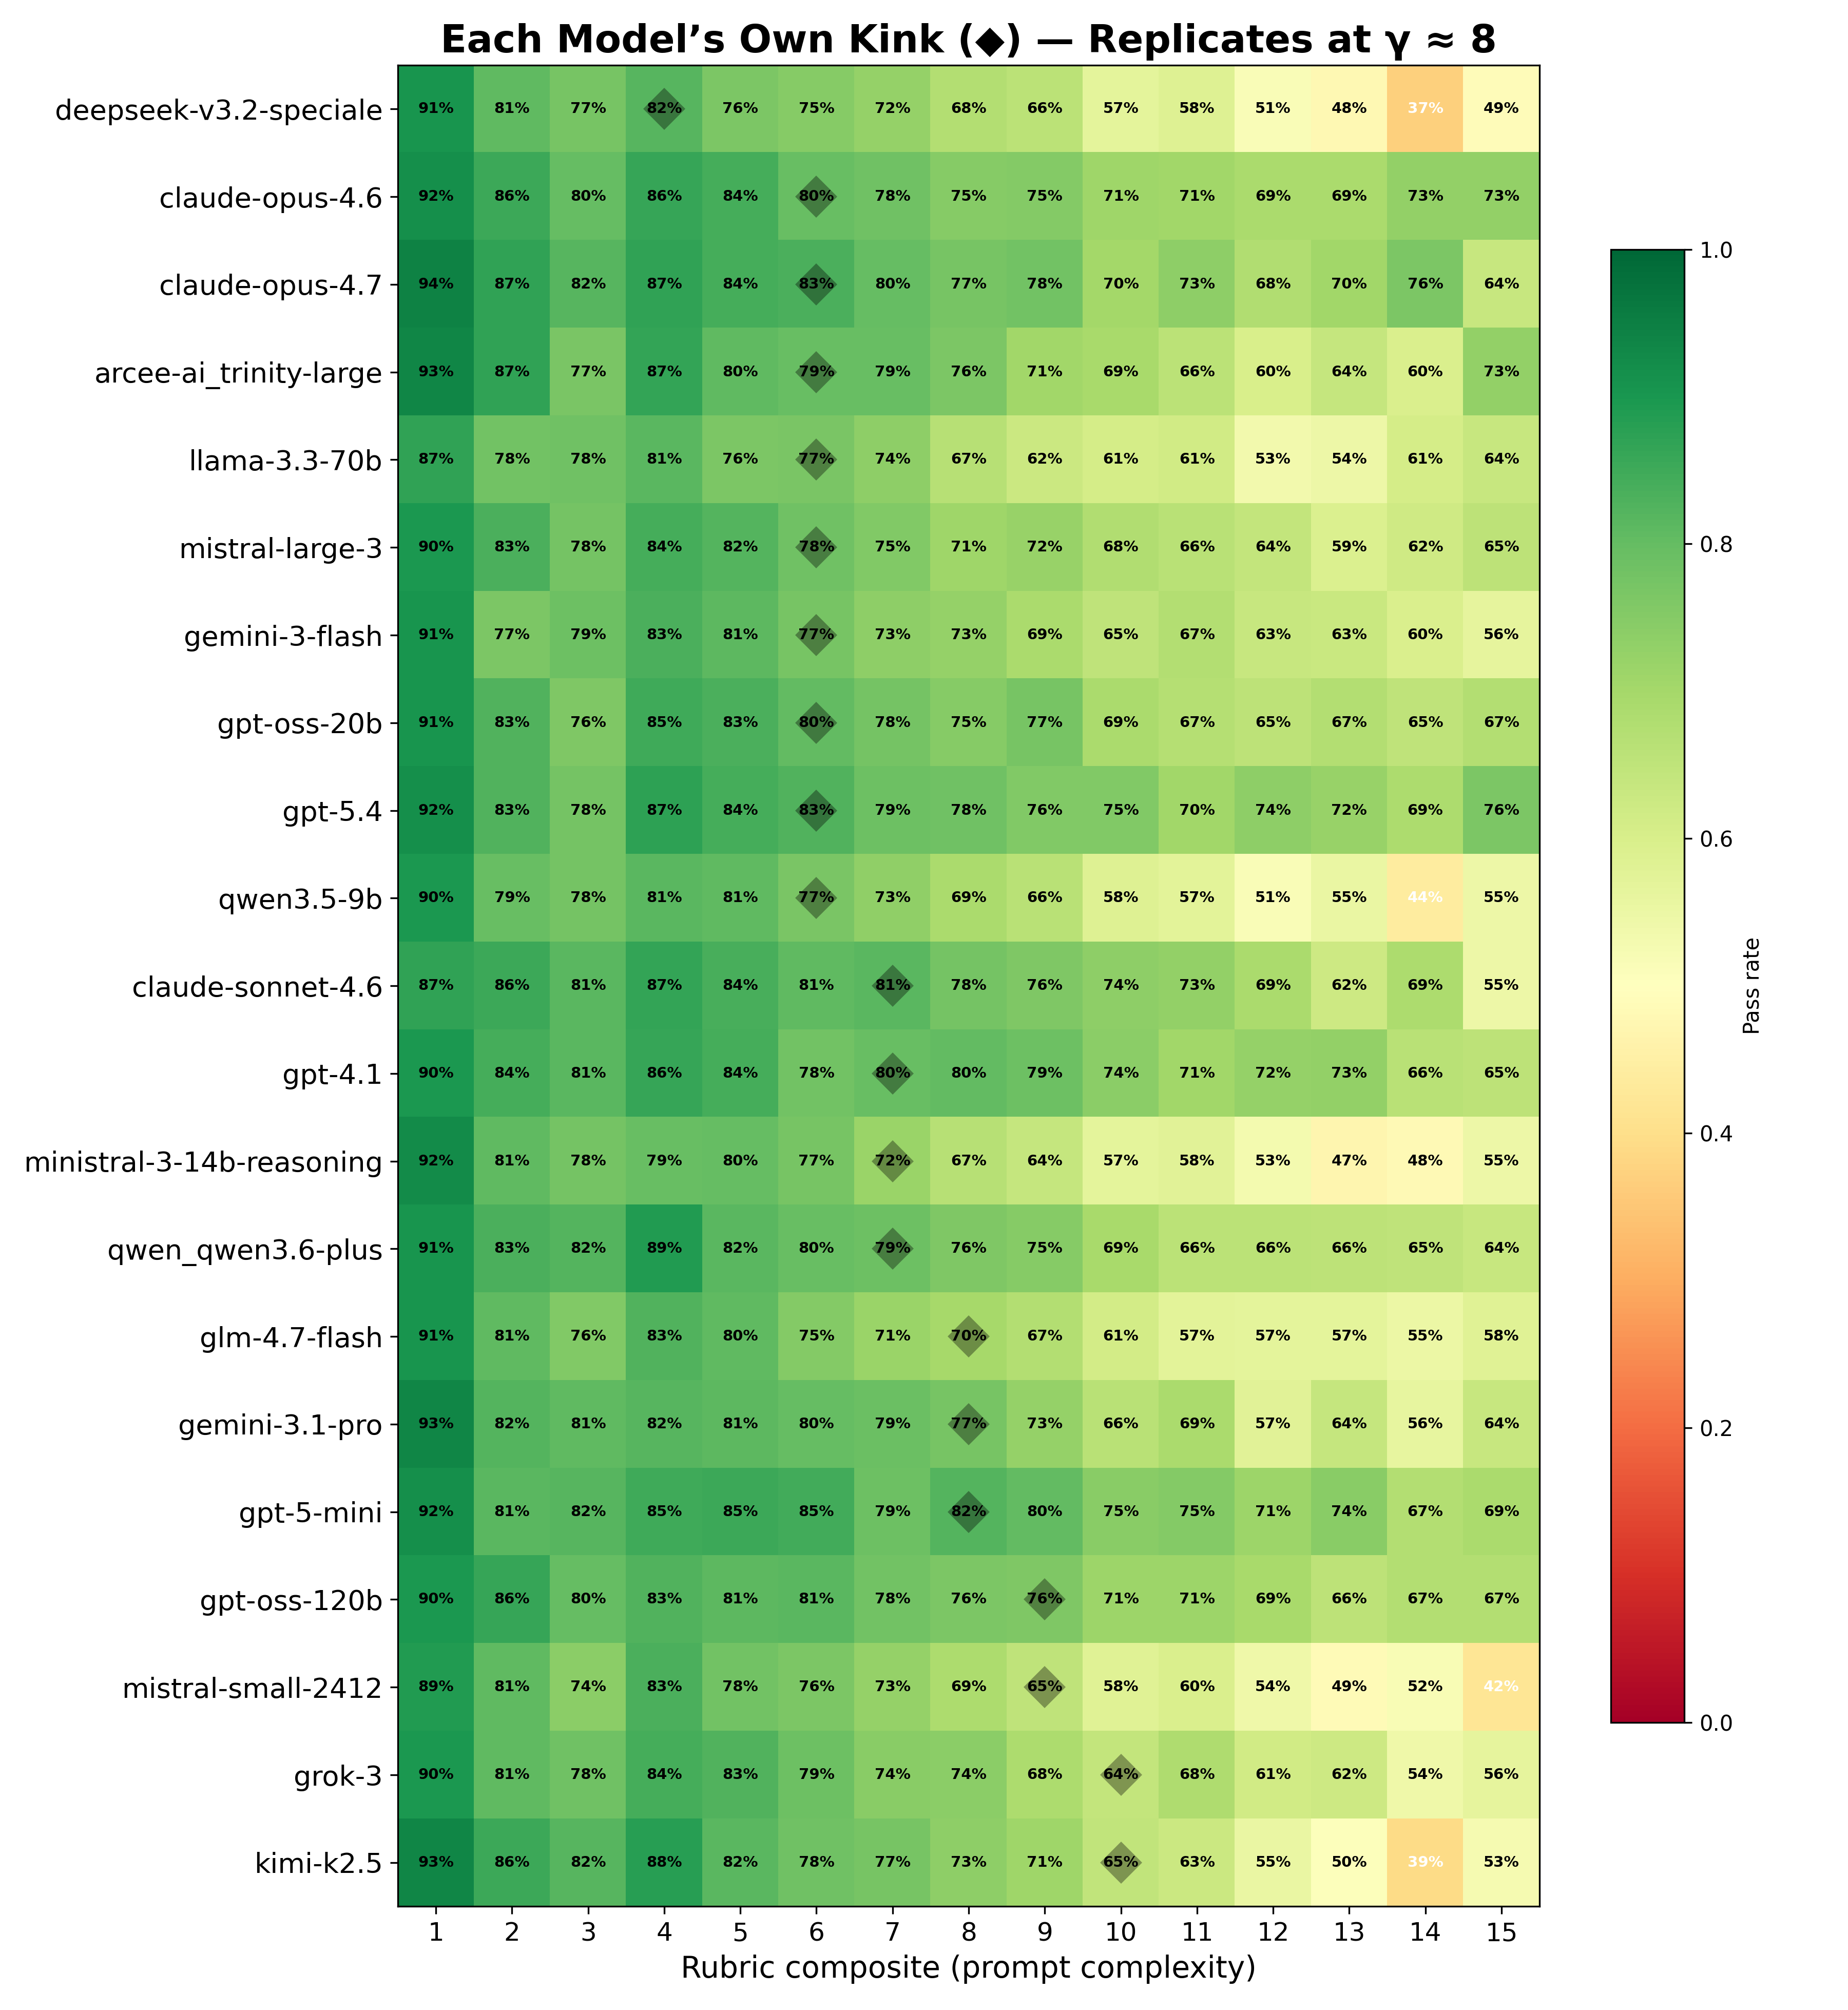
\includegraphics[width=\columnwidth]{../figures/per_model_kink_heatmap.png}
\caption{Per model Hansen sup Wald surface. Rows are the 21 panel models, columns are candidate $\gamma$ values. Cell color indicates $W(\gamma)$ for that model. Each row's maximum is annotated with a marker. The strongest models (Grok-3, Kimi K2.5) locate their individual $\hat{\gamma}$ at the right of the grid near 10, while the bulk of models cluster near $\hat{\gamma}=6$.}
\label{fig:heatmap}
\end{figure}

\begin{table}[h]
\centering
\caption{Per model threshold estimates. Pass rates split at each model's individual $\hat{\gamma}$. Hansen $p$ and placebo $p$ are the bootstrap threshold test and 500 iteration shuffled $\hat{\kappa}$ test, respectively.}
\label{tab:per-model}
\small
\begin{tabular}{@{}lrrrrr@{}}
\toprule
Model & $\hat{\gamma}$ & Pass $<\hat{\gamma}$ & Pass $\geq\hat{\gamma}$ & Hans $p$ & Plcb $p$ \\
\midrule
Claude Opus 4.6          & 6.0  & 52.0\% & 38.2\% & $<$.001 & $<$.001 \\
Claude Opus 4.7          & 6.0  & 53.9\% & 40.8\% & $<$.001 & $<$.001 \\
Claude Sonnet 4.6        & 7.0  & 48.1\% & 36.9\% & $<$.001 & $<$.001 \\
Trinity-large            & 6.0  & 58.4\% & 44.5\% & $<$.001 & $<$.001 \\
DeepSeek V3.2            & 4.0  & 52.4\% & 36.0\% & 0.10    & 0.13 \\
GPT-OSS-120B             & 9.0  & 46.2\% & 37.3\% & $<$.001 & $<$.001 \\
Grok-3                   & 10.0 & 44.6\% & 33.5\% & $<$.001 & $<$.001 \\
Kimi K2.5                & 10.0 & 41.7\% & 27.8\% & 0.01    & 0.02 \\
Llama 3.3-70B            & 6.0  & 53.5\% & 40.3\% & 0.05    & 0.08 \\
Mistral Large-3          & 6.0  & 56.0\% & 41.0\% & $<$.001 & 0.01 \\
GLM 4.7-flash            & 8.0  & 48.3\% & 37.1\% & $<$.001 & $<$.001 \\
Gemini 3 Flash           & 6.0  & 54.9\% & 39.1\% & $<$.001 & $<$.001 \\
Gemini 3.1 Pro           & 8.0  & 50.8\% & 38.8\% & $<$.001 & $<$.001 \\
GPT-4.1                  & 7.0  & 51.2\% & 40.3\% & $<$.001 & $<$.001 \\
GPT-5-mini               & 8.0  & 52.2\% & 40.2\% & $<$.001 & $<$.001 \\
GPT-OSS-20B              & 6.0  & 54.1\% & 39.0\% & $<$.001 & $<$.001 \\
Ministral-3-14B-rsn      & 7.0  & 50.1\% & 36.5\% & $<$.001 & $<$.001 \\
Mistral Small 2412       & 9.0  & 46.2\% & 34.2\% & $<$.001 & $<$.001 \\
GPT-5.4                  & 6.0  & 56.6\% & 42.0\% & $<$.001 & $<$.001 \\
Qwen 3.5-9B              & 6.0  & 54.1\% & 39.3\% & $<$.001 & $<$.001 \\
Qwen 3.6 Plus            & 7.0  & 52.4\% & 38.3\% & $<$.001 & $<$.001 \\
\midrule
Combined (21 models)     & 8.0  & 47.9\% & 35.9\% & $<$.001 & $<$.001 \\
\bottomrule
\end{tabular}
\end{table}

\subsection{Frontier vs.\ Open Source Gap}

Figure~\ref{fig:gap} shows that the performance gap between frontier and open source models widens as rubric complexity increases. Easy tasks compress the gap, and hard tasks separate models. At the kink the gap widens sharply. This is consistent with the interpretation that the Complexity Kink is the point at which model capability differences begin to matter for deployment.

\begin{figure}[h]
\centering
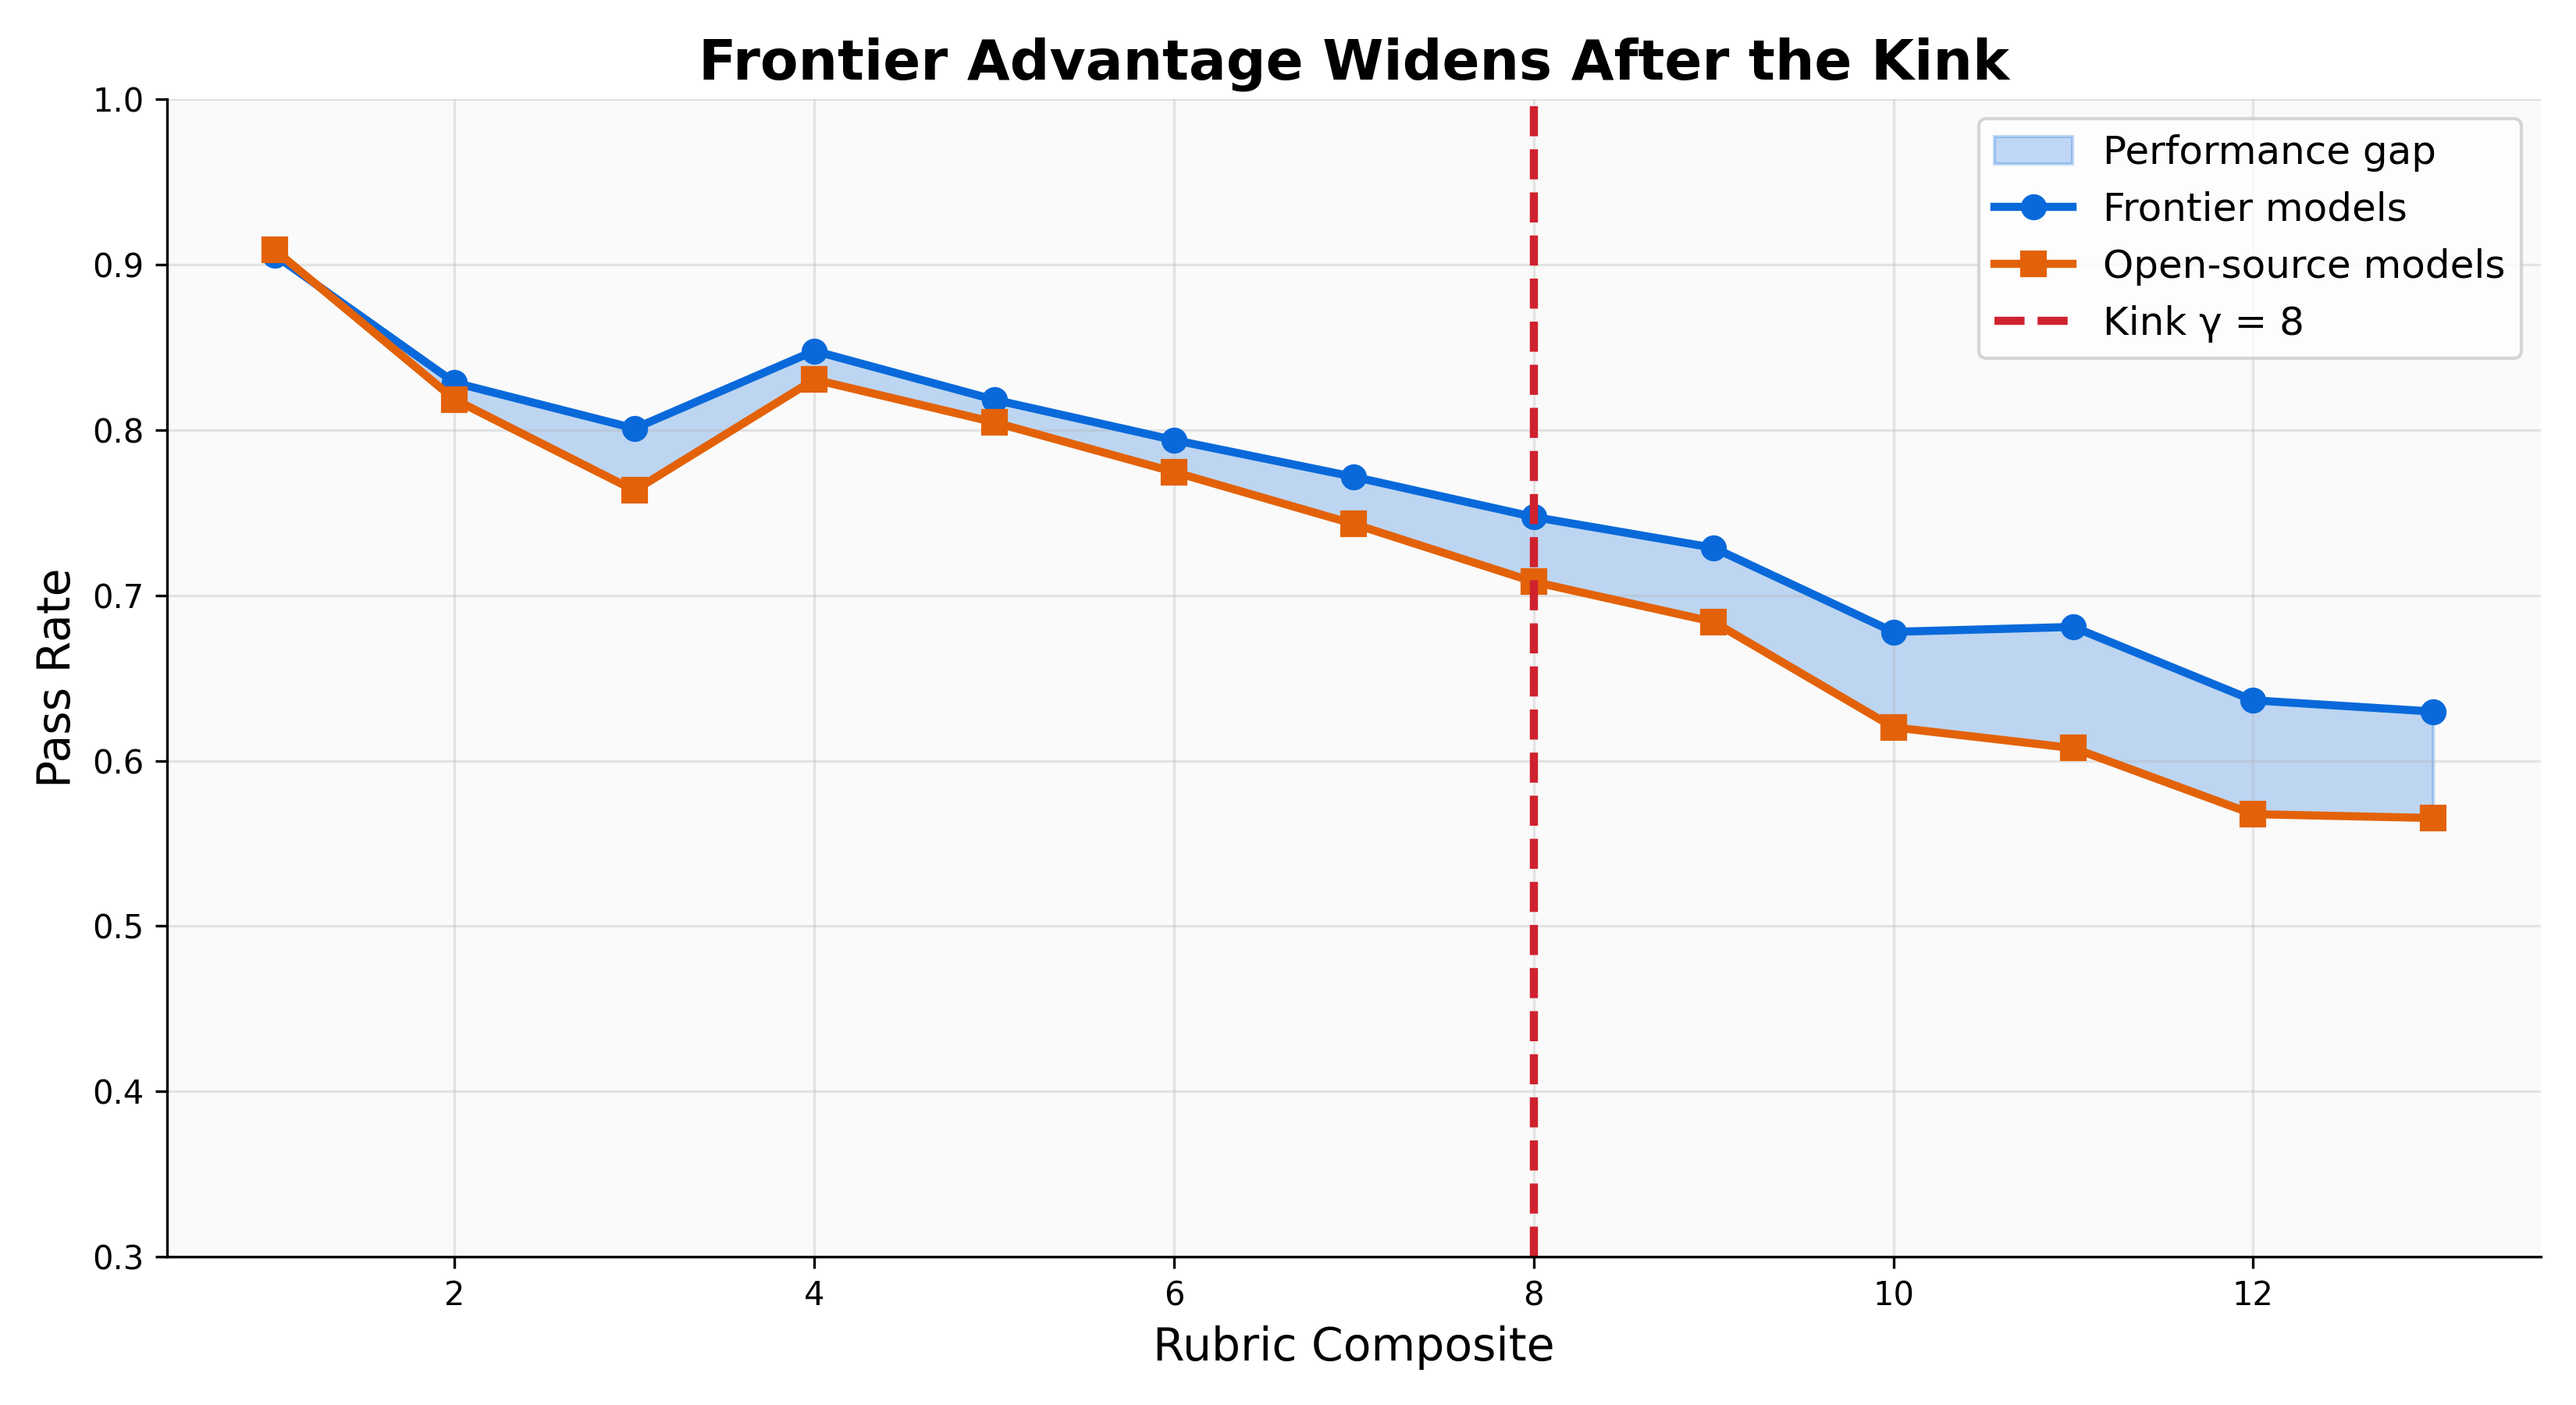
\includegraphics[width=\columnwidth]{../figures/frontier_vs_open_source_gap.png}
\caption{Frontier advantage widens after the kink. Mean pass rate for frontier ($n=14$) and open source ($n=6$) model subsets against rubric composite. Vertical dashed line: $\hat{\gamma}\approx 8.0$.}
\label{fig:gap}
\end{figure}

\subsection{Dimension Level Performance}

Figure~\ref{fig:radar} decomposes model performance on hard tasks (rubric composite $\geq 3$ per dimension) across the six rubric dimensions. Frontier models dominate on branching and iteration, the two dimensions anchored most directly to control flow, and compress toward open source performance on state and composition, the dimensions requiring coordination across algorithmic steps.

\begin{figure}[h]
\centering
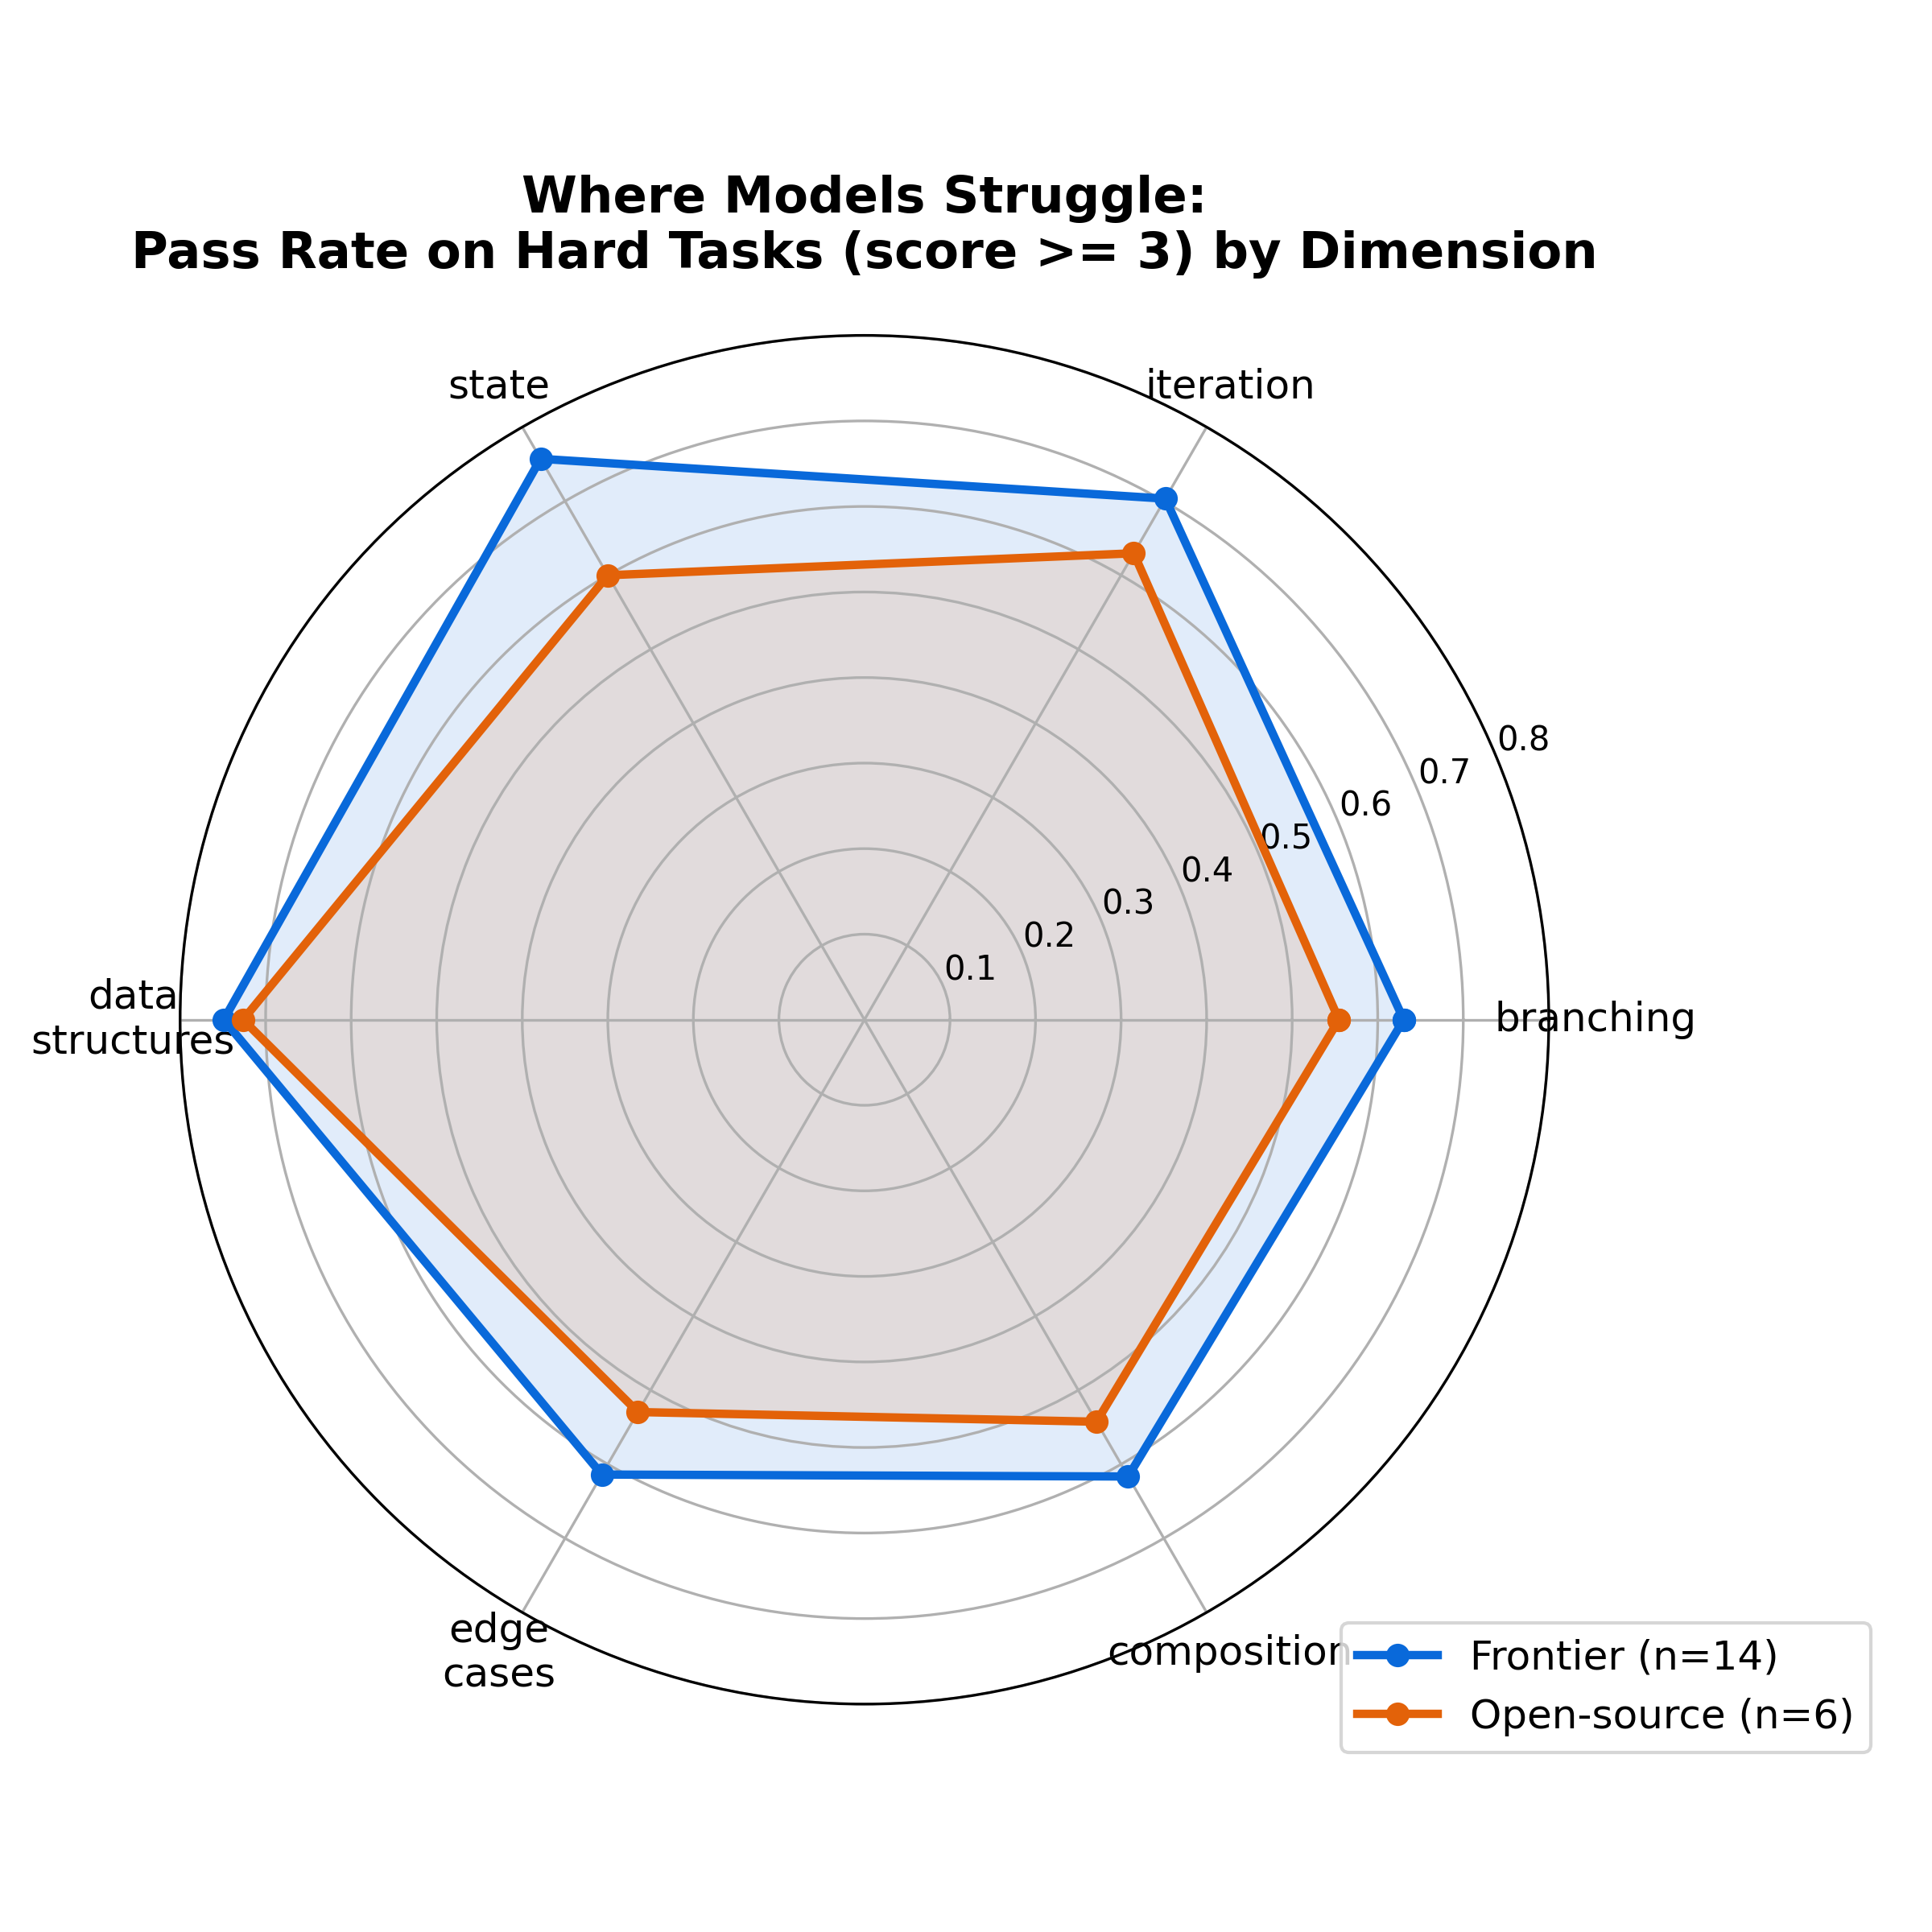
\includegraphics[width=\columnwidth]{../figures/dimension_performance_radar.png}
\caption{Dimension level performance on hard tasks (dimension score $\geq 3$). Frontier models ($n=14$) compared with open source ($n=6$). The frontier advantage is largest on branching and iteration, smallest on state and composition.}
\label{fig:radar}
\end{figure}

\subsection{Sankey: Visualizing the Reverse Threshold Problem}

Figure~\ref{fig:sankey} visualizes the mechanism underlying the benchmark bias. Tasks flow from their true (rubric) complexity on the right to their observed output CC bin on the left. Red flows are tasks that are complex by rubric but register as $\kappa^{\text{obs}}=1$ by output, which is the contamination that drives the Reverse Threshold Problem. Approximately 2\% of the dataset routes through the red flow, the same bias the Stage~B paper first quantified and which the Stage~C rubric instrument now isolates.

\begin{figure}[h]
\centering
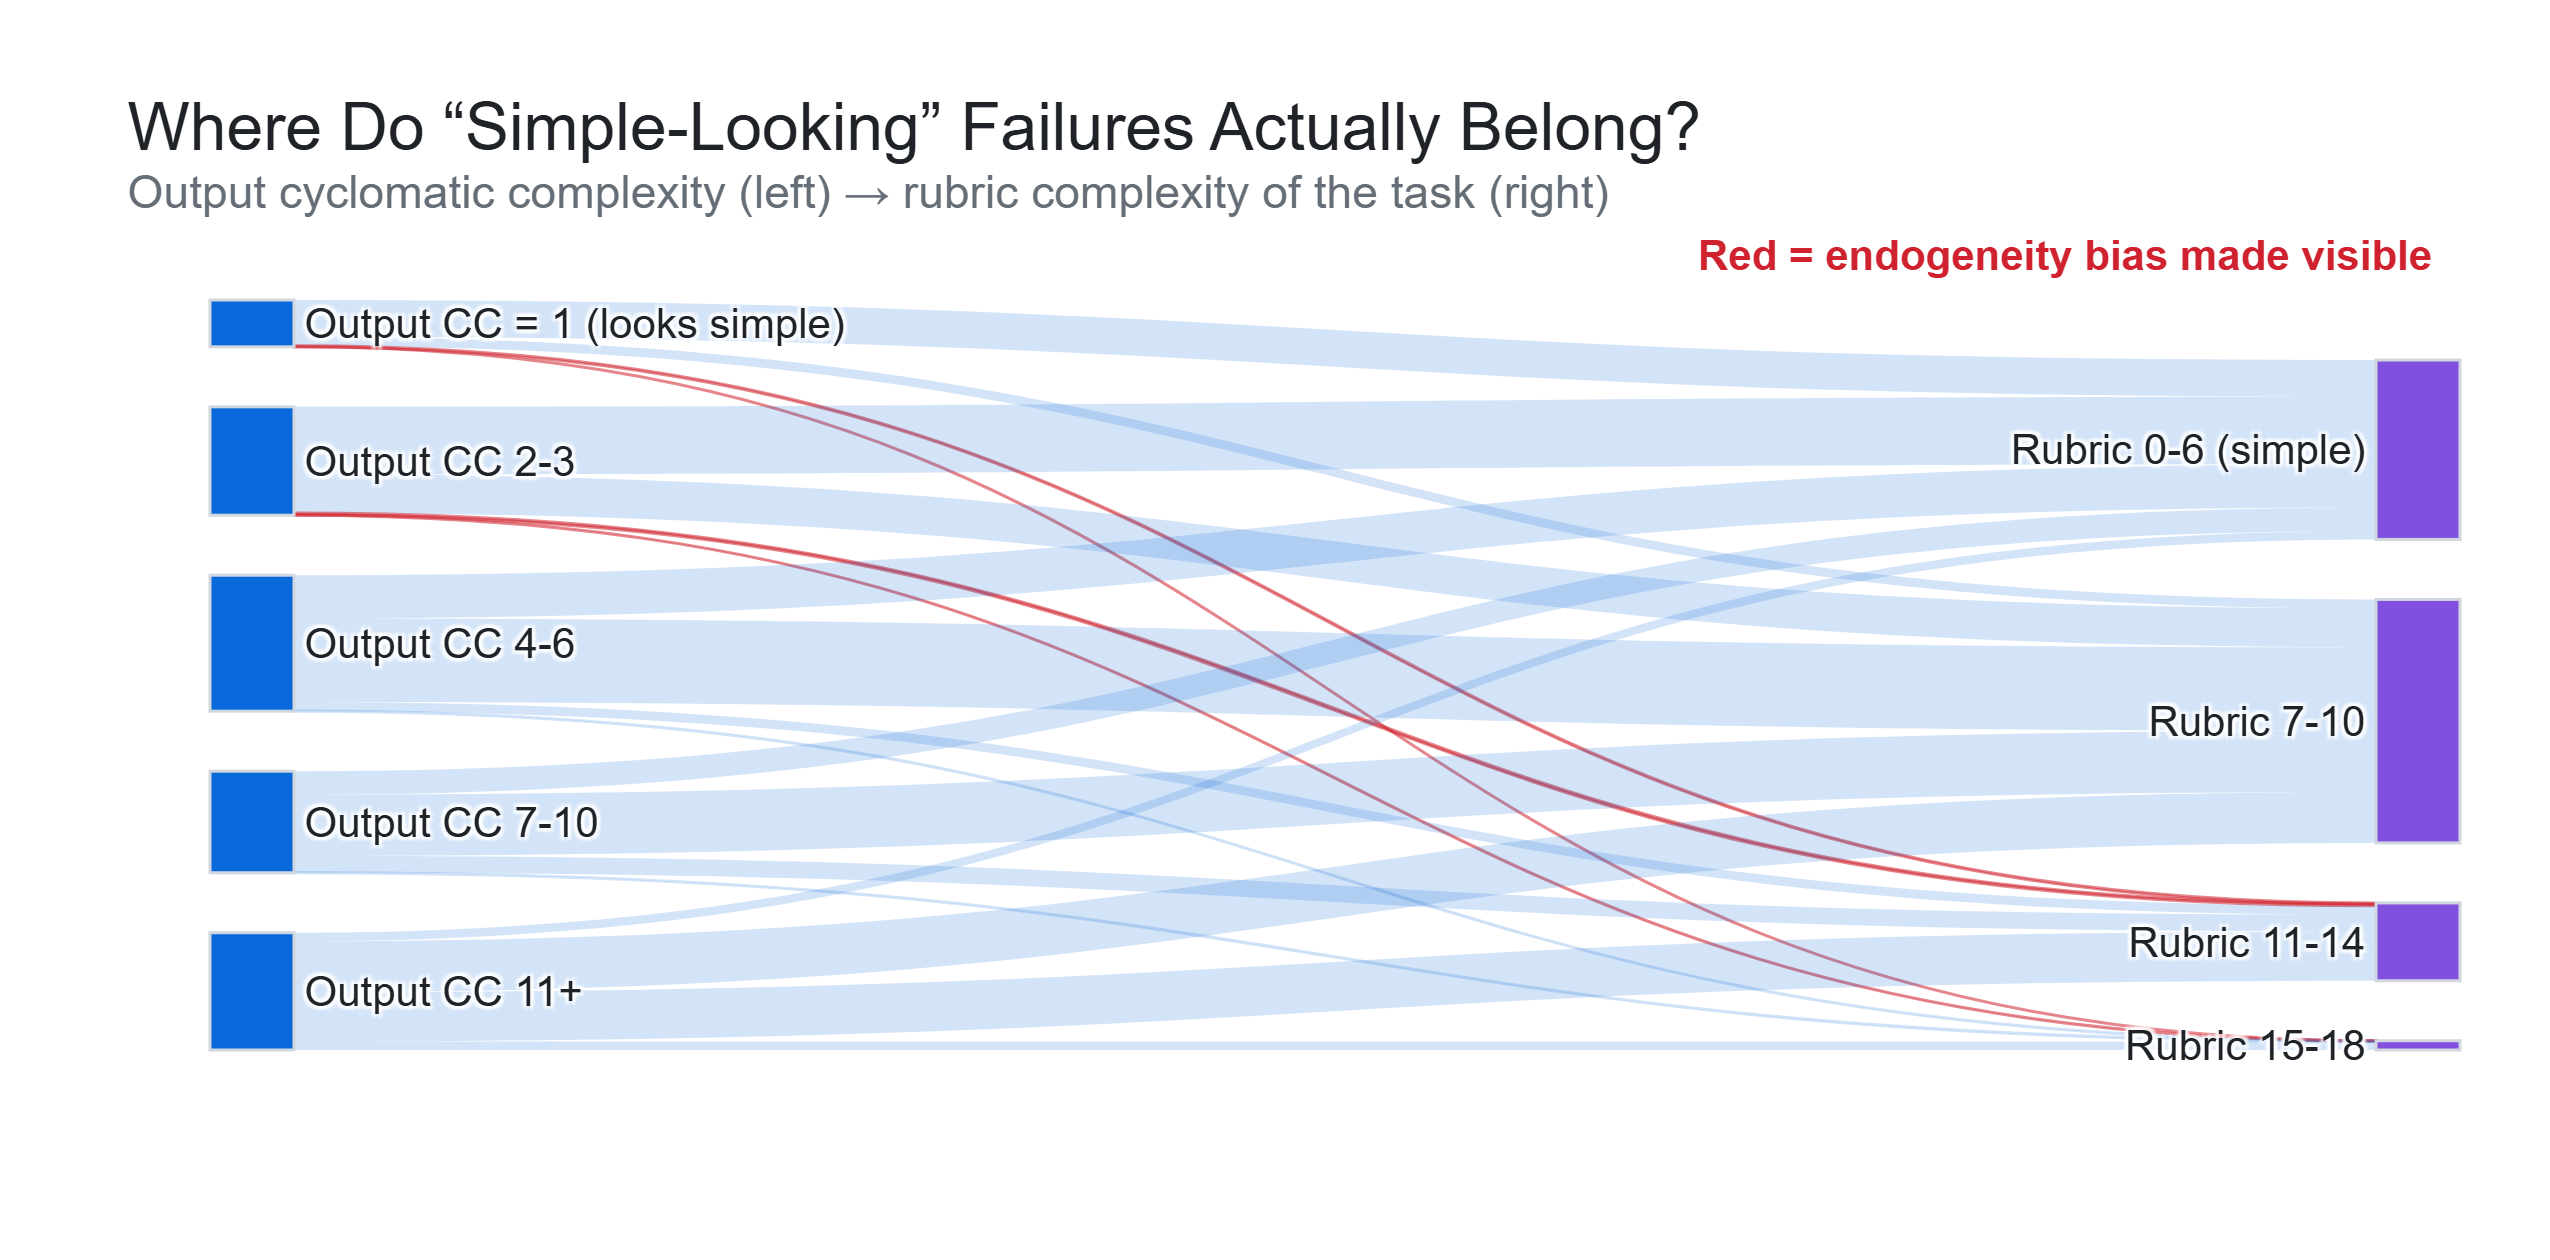
\includegraphics[width=\columnwidth]{../figures/sankey_misclassification.png}
\caption{Reverse Threshold Problem visualized. Tasks flow from observed output cyclomatic complexity (left) to rubric complexity of the task (right). Red flows mark endogenously biased misclassifications: complex tasks whose failure produced output with $\kappa^{\text{obs}}=1$.}
\label{fig:sankey}
\end{figure}

\subsection{Placebo}

Across 500 placebo iterations (shuffled rubric composite) on the combined dataset, the mean placebo sup Wald is $2.22$ (SD $1.27$) with 95\% range $[0.51, 5.22]$ and maximum $9.04$. The observed $W^*=12.08$ at $\hat{\gamma}=8.0$ exceeds every single placebo draw ($p<0.002$); the observed value sits $7.7$ standard deviations above the placebo mean. The identified break is therefore highly unlikely to be a statistical artifact of the Hansen grid search. In the per model placebo, 19 of 21 panel models similarly reject the null at the 5\% level, with the same two exceptions (DeepSeek V3.2, Llama 3.3-70B) that were marginal under the Hansen bootstrap.

\begin{figure}[h]
\centering
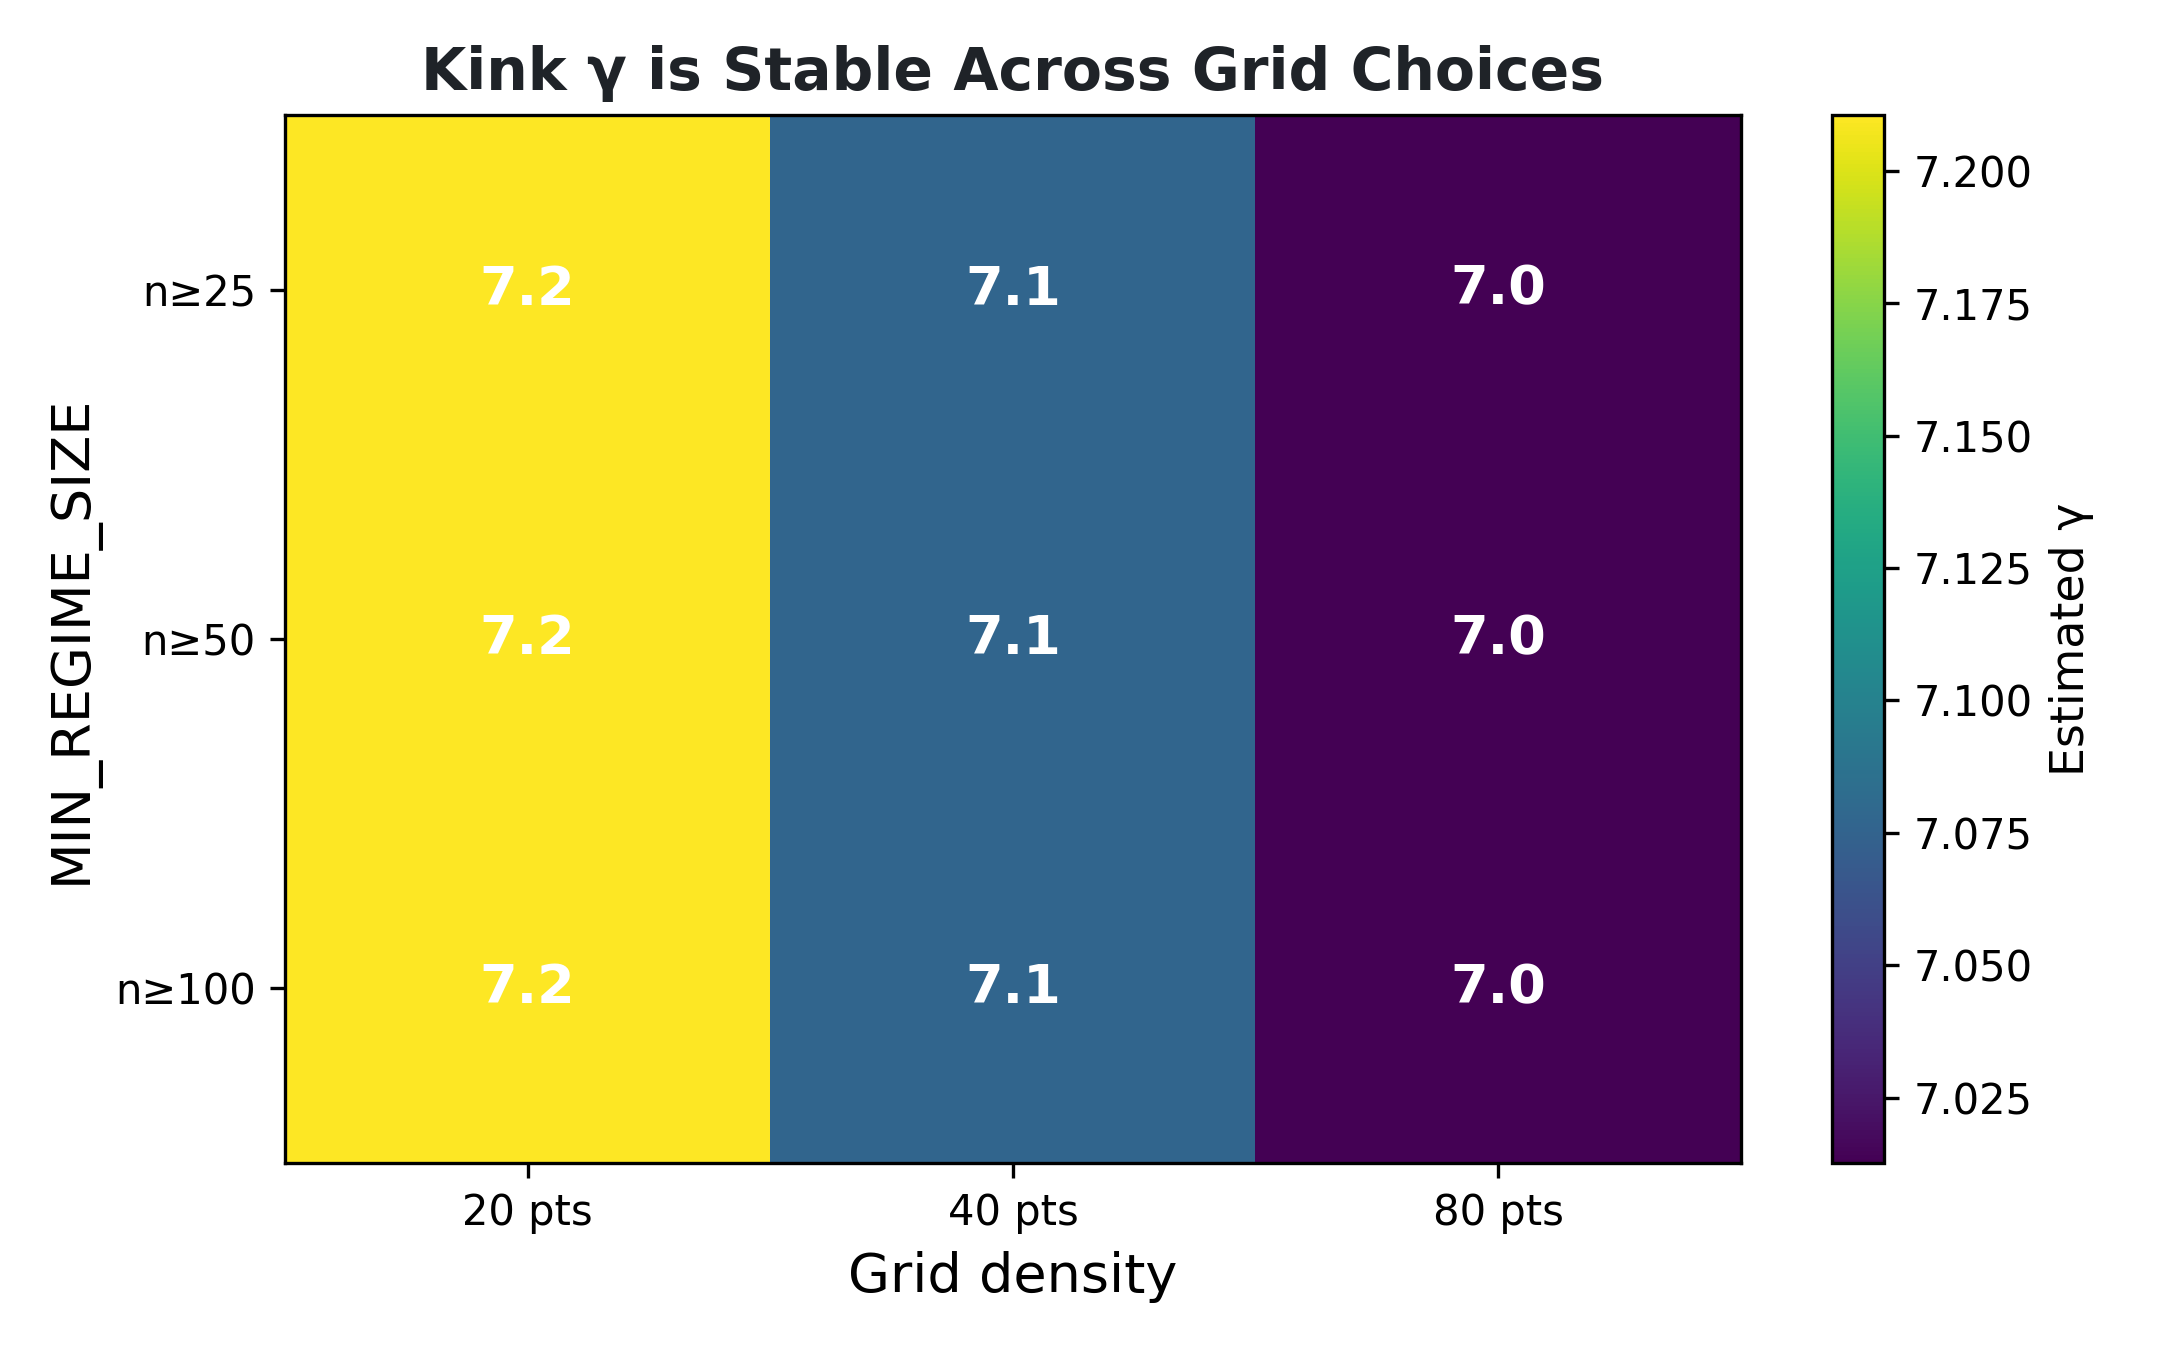
\includegraphics[width=\columnwidth]{../figures/threshold_sensitivity.png}
\caption{Sensitivity of $\hat{\gamma}$ to \texttt{MIN\_REGIME} (minimum sample size per regime) and Hansen grid density. Bars indicate 95\% bootstrap CI on $\hat{\gamma}$ at each configuration. Estimate is stable across the configuration space.}
\label{fig:sensitivity}
\end{figure}

\subsection{Sparse Tail Caveat}

At rubric composite $\geq 15$, per bin sample sizes drop sharply: $n=1{,}047$ at composite 15, $476$ at 16, $152$ at 17, $38$ at 18 (pooled across the 21 panel models). Within this sparse tail, the combined pass rate curve exhibits a non monotone bump from $\approx$31\% at composite~15 to $\approx$50\% at composite~16 before collapsing to $\approx$3\% at composite~18. Inspection of the prompts indicates that composite~$\geq$~16 prompts are disproportionately framework requiring tasks (ML pipelines, parsers, compilers) whose correct solution often reduces to a library call (\texttt{transformers.pipeline}, \texttt{sklearn.Pipeline}). The failure mode shifts from ``can the model reason'' to ``does the model know the library.'' Accordingly, all combined curve figures in this paper restrict to bins with $n\geq 1{,}000$. The main estimate of $\hat{\gamma}\approx 8$ is located in the dense mid range and is not sensitive to this tail.

% =====================================================================
\section{Discussion}
% =====================================================================

\subsection{The Exclusion Restriction under Rubric Instruments}

The identifying assumption is that each rubric dimension $Z_{i,d}$ affects $y_i$ \emph{only through} $\kappa_i^*$, that is, $\mathrm{Cov}(Z_{i,d}, u_i)=0$. We defend this claim on four grounds.

\textbf{Rubric design.} Each dimension is anchored to artifacts of the correct code structure (branches, loops, state variables), not to constructs that would have independent channels to $y_i$ such as task novelty, prompt ambiguity, or library obscurity. The system prompt explicitly instructs the scorer to score the structure of the correct solution, not the difficulty of understanding.

\textbf{Scorer exclusion.} The scorer (o4-mini) is not in the evaluated panel. A scorer specific bias such as systematic over scoring of edge case dimensions would affect all 21 panel models in the level, not the slope of the pass rate relationship, and the exclusion restriction survives up to a constant shift.

\textbf{Over identification test.} The Sargan and Hansen $J$ rejects the joint null of valid exclusion ($p\approx 0$ on the combined dataset; see \S\ref{sec:hansen-j}). The honest reading is that at least one of the six dimensions has a residual direct correlation with the error term. The size of the $p$-value is consistent with a pattern common to very large samples in over identified IV~\cite{bowsher2002reject}, where even small violations produce strong rejections. We do not treat the $p$-value as dispositive, but we also do not claim it provides positive support for exclusion; it does not. The consequence is that the 2SLS point estimate of $\beta$ should be read as an upper bound, under the ensuing ensemble design (\S\ref{sec:stage-d}) we can decompose scorer specific noise from structural signal and tighten the identification argument.

\textbf{Acknowledgment of untestability.} As with every IV design, the exclusion restriction cannot be proven by test alone; the $J$ statistic detects disagreement across instruments, not common mode violations. We flag single scorer idiosyncrasy as the largest remaining vulnerability and propose Stage~D (\S\ref{sec:stage-d}) as a direct mitigation.

\subsection{Elimination of Stage~B's Remaining Weaknesses}

Table~\ref{tab:b-vs-c} compares Stage~B and Stage~C on each of the four Stage~B weaknesses.

\begin{table}[h]
\centering
\caption{Stage~B (keyword RF) compared with Stage~C (LLM rubric) on Stage~B's known weaknesses.}
\label{tab:b-vs-c}
\begin{tabular}{@{}lll@{}}
\toprule
Issue & Stage~B & Stage~C \\
\midrule
Survivorship bias        & Present & \textbf{Eliminated} \\
Generated regressor      & Present & \textbf{Eliminated} \\
$\kappa=1$ vs $\kappa=2$ & n.s.    & $p<10^{-6}$ \\
Monotone instruments     & 6 of 8  & \textbf{6 of 6} \\
Number of instruments    & 8       & 6 \\
$J$ test interpretable   & No      & Yes (rejects) \\
First stage $F$          & 1{,}765 & 2{,}926 \\
Hausman $\chi^2$         & 108.5   & 24.5 \\
\bottomrule
\end{tabular}
\end{table}

\subsection{LLM Rubric Scoring as a New Class of Instruments}

IV estimation in empirical economics, epidemiology, and the social sciences is frequently constrained by instrument availability. Finding a variable that predicts the endogenous regressor without opening a direct channel to the outcome is often the binding constraint on causal identification. The Stage~C framework introduces a new class of instruments: LLM scored rubric dimensions over text artifacts, with the scorer excluded from the evaluated population. The construction generalizes naturally beyond code generation. Any setting in which the endogenous covariate is latent inside a text artifact (clinical notes predicting diagnostic severity, legal filings predicting outcomes, review text predicting customer behavior) admits a rubric scoring approach. We expect this approach will prove practically useful for IV work in domains where traditional instruments have been hard to find.

\subsection{Implications for Benchmark Design}
If the Stage~C results generalize, current LLM code generation benchmarks, which report aggregate pass rates over output derived complexity bins, may overstate reliability on structurally complex tasks. We recommend that benchmark designers (a) report pass rates stratified by input derived complexity (rubric or equivalent), (b) publish the scoring rubric and scorer identity for reproducibility, and (c) test for structural breaks in the relationship between complexity and pass rate rather than fitting smooth parametric curves.

% =====================================================================
\section{Limitations and Stage~D}
\label{sec:stage-d}
% =====================================================================

\subsection{Limitations of Stage~C}

\textbf{Single scorer rubric.} The instrument is constructed by a single LLM (o4-mini). Any private bias of the scorer, such as systematic over or under scoring of a specific dimension, propagates into every instrument observation, and cannot be measured or corrected within Stage~C's design.

\textbf{Sampling stratification inherits the output endogeneity problem.} The 5{,}000 prompt sample was stratified across reference cyclomatic complexity bins computed by \texttt{lizard} on the Qwen2.5 reference solution. This carries the same endogeneity the main analysis corrects for, but at the sampling layer: a prompt where the reference solver failed receives a low \texttt{reference\_cc} and is binned as ``simple,'' causing the sample to systematically undersample prompts at the complex tail. The effect is that $\hat{\gamma}$ and the kink magnitude are estimated on a sample with fewer truly complex prompts than the full OpenCodeInstruct pool contains. Stage~D corrects this by stratifying on rubric composite rather than on \texttt{reference\_cc}.

\textbf{Python only.} Stage~B demonstrated the Complexity Kink across Python, JavaScript, Go, Java, and C++. Stage~C restricts to Python for tractable scoring and consistent unit test execution. Cross language replication with the rubric instrument is the most direct generalization.

\textbf{Exclusion restriction untestable in isolation.} The Sargan and Hansen $J$ test can detect disagreement across instruments but cannot detect a \emph{common mode} violation in which every rubric dimension equally picks up a direct channel to $y_i$. The argument against common mode violations is therefore a claim about design rather than a test.

\textbf{Cross sectional only.} We demonstrate the kink exists, but we do not track $\hat{\gamma}$ across model generations. Whether frontier progress moves $\hat{\gamma}$ rightward over time is an open question.

\subsection{Stage~D: Rubric Stratified Resampling, Ensemble Scoring, and Errors in Variables Correction}

Stage~D, planned as the next iteration, addresses three separate Stage~C limitations with a single integrated design.

\subsubsection{Component 1: Rubric stratified resampling}
The Stage~C sample inherits an output endogeneity at the stratification layer: bins are defined on \texttt{reference\_cc}, the cyclomatic complexity of the Qwen2.5 reference solution, which collapses toward 1 when the reference solver failed on a genuinely complex prompt. Stage~D will score a large sub-pool of OpenCodeInstruct (target: $\geq 50{,}000$ prompts, budget permitting) with the published rubric, then stratify by rubric composite rather than by \texttt{reference\_cc} to draw a new 5{,}000 prompt sample. The resulting sample will have tail coverage determined entirely by the structural complexity of the prompt, free of reference-solver failure contamination.

This is a direct methodological parallel to the main analysis: the rubric removes output endogeneity from the Stage~2 structural regressor, and Stage~D extends the same fix into the sampling frame. We expect this to shift $\hat{\gamma}$ and widen the estimated kink drop, because the current sample systematically undersamples the tail where the pass rate collapses.

\subsubsection{Component 2: Ensemble rubric across four scorers}
The most direct mitigation of single scorer idiosyncrasy is to score each prompt with multiple frontier LLMs, all excluded from the evaluated panel, and report inter rater reliability. Stage~D will score every prompt in the rubric stratified sample with four frontier scorers (o4-mini, plus three additional models that are not in the panel), reporting Cohen's $\kappa$ and ICC across scorers. The ensemble composite replaces o4-mini's single score as the instrument.

\subsubsection{Component 3: Errors in variables correction}
Between scorer variance $\hat{\sigma}^2_{\text{scorer}}$ is computed per prompt from the four scorer ensemble. This is a \emph{measured} estimate of instrument measurement error and can be fed into the 2SLS first stage as a direct errors in variables correction of Stage~1 coefficients. In applied IV, $\hat{\sigma}^2_{\text{u}}$ on the instrument is almost never available; Stage~D has it because the instrument is constructed, not found.

\subsubsection{Component 4: Human scored calibration subsample}
A 500 prompt subsample will be hand scored by the author against the published rubric, blind to LLM outputs. Human versus ensemble agreement serves as an external validity check and as a bound on LLM-specific biases shared across scorers.

The joint Stage~D design targets three limitations simultaneously: sampling frame endogeneity (Component 1), single scorer idiosyncrasy (Components 2 and 4), and unmeasured instrument noise (Component 3). If the Sargan and Hansen $J$ rejection in Stage~C is driven by single scorer bias, the ensemble in Component 2 should attenuate it; if it is driven by a common mode violation across all LLM scorers, the human subsample in Component 4 will detect it.

% =====================================================================
\section{Related Work}
% =====================================================================

\textbf{LLM code evaluation.} HumanEval~\cite{chen2021evaluating}, MBPP~\cite{austin2021program}, and SWE-Bench~\cite{jimenez2023swebench} are the dominant benchmarks. All measure difficulty from output characteristics. DevBench, Mostly Basic Python, and CodeContests follow the same pattern. None, to our knowledge, correct for the endogeneity we identify.

\textbf{IV in software engineering.} IV has been applied sporadically in software engineering. McIntosh et al.~\cite{mcintosh2016empirical} instrument for code review effects on defects. Mockus~\cite{mockus2010organizational} instruments for organizational volatility on defects. Our Stage~B~\cite{hernandez2026complexity} was, to our knowledge, the first application to LLM code evaluation. Stage~C extends the framework with LLM scored rubric instruments.

\textbf{Threshold regression.} Hansen's sup Wald threshold test~\cite{hansen2000sample} and its bootstrap extension are standard in empirical macroeconomics (tax thresholds, currency regime transitions) but rare in software engineering research.

\textbf{LLM as judge literature.} G-Eval~\cite{liu2023geval}, AlpacaEval~\cite{alpacaeval}, and MT-Bench~\cite{zheng2023judging} use LLMs to score open ended outputs. Our usage differs: rather than scoring LLM outputs (and thereby inheriting output endogeneity), we score \emph{task prompts}, using the LLM to construct an instrument rather than to evaluate. We are not aware of prior work in this direction.

\textbf{Rubric scoring in NLP evaluation.} Rubric based automatic evaluation has precedent in NLP~\cite{hashimoto2019unifying}. Our contribution is to embed rubric scoring inside an IV identification strategy rather than to use it as a standalone metric.

% =====================================================================
\section{Conclusion}
% =====================================================================

The Complexity Kink is a property of the code generation task distribution, not an artifact of any specific instrument or model. Under a stronger identification strategy, namely a six dimension LLM scored rubric that eliminates the survivorship bias and generated regressor problems of the Stage~B keyword RF instrument, we replicate the structural break at $\hat{\gamma}=8.0$ on the composite rubric scale, with below kink pass rate 48.9\% and above kink 37.0\%. The kink replicates at the 5\% level in 19 of 21 frontier models from 2025 and 2026, with the qualitative decline present in all 21. The Sargan and Hansen $J$ test rejects joint exclusion, which we read as a honest flag on single scorer idiosyncrasy; the Stage~D ensemble scoring extension is designed to address this directly.

For practitioners: deploying LLM generated code near or above rubric composite 8 warrants additional human review. Reliability above this threshold is substantially below the headline pass rates reported on output based benchmarks.

For benchmark designers: input derived complexity scoring should replace or supplement output derived metrics in future LLM code generation benchmarks.

For the IV methodology literature: LLM scored rubrics constitute a novel and general class of instruments for endogenous covariates that live inside text.

\vspace{4pt}
\noindent\textbf{Reproducibility.} All code, rubric system prompts, rubric scores, and analysis scripts are available at \url{https://github.com/mhernandez2026/ComplexityKinkResearch}.

\noindent\textbf{Acknowledgments.} The author thanks Dr.\ Tian Zhao, faculty advisor, Department of Computer Science, UWM, and the UWM Connected Systems Institute for Azure compute support covering rubric scoring and evaluated panel inference costs.

% =====================================================================
\bibliographystyle{IEEEtranN}
\begin{thebibliography}{99}

\bibitem{hernandez2026complexity}
M.~Hernandez, ``The Complexity Kink: Identifying a Hard Reliability Threshold in LLM Code Generation via Instrumental Variables,'' preprint, 2026.

\bibitem{chen2021evaluating}
M.~Chen et al., ``Evaluating Large Language Models Trained on Code,'' \emph{arXiv:2107.03374}, 2021.

\bibitem{austin2021program}
J.~Austin et al., ``Program Synthesis with Large Language Models,'' \emph{arXiv:2108.07732}, 2021.

\bibitem{opencodeinst}
NVIDIA, ``OpenCodeInstruct,'' Hugging Face Datasets, 2025.

\bibitem{wooldridge2010econometric}
J.~M.~Wooldridge, \emph{Econometric Analysis of Cross Section and Panel Data}, 2nd~ed., MIT Press, 2010.

\bibitem{hansen2000sample}
B.~E.~Hansen, ``Sample Splitting and Threshold Estimation,'' \emph{Econometrica}, vol.~68, no.~3, pp.~575 to 603, 2000.

\bibitem{hansen1982large}
L.~P.~Hansen, ``Large Sample Properties of Generalized Method of Moments Estimators,'' \emph{Econometrica}, vol.~50, no.~4, pp.~1029 to 1054, 1982.

\bibitem{jimenez2023swebench}
C.~E.~Jimenez et al., ``SWE-bench: Can Language Models Resolve Real-World GitHub Issues?'' \emph{arXiv:2310.06770}, 2023.

\bibitem{mcintosh2016empirical}
S.~McIntosh et al., ``An Empirical Study of the Impact of Modern Code Review Practices on Software Quality,'' \emph{Empirical Software Engineering}, vol.~21, no.~5, pp.~2146 to 2189, 2016.

\bibitem{mockus2010organizational}
A.~Mockus, ``Organizational Volatility and Its Effects on Software Defects,'' in \emph{Proc.\ 18th ACM SIGSOFT Int.\ Symp.\ Foundations of Software Engineering (FSE)}, 2010, pp.~117 to 126.

\bibitem{liu2023geval}
Y.~Liu et al., ``G-Eval: NLG Evaluation using GPT-4 with Better Human Alignment,'' \emph{arXiv:2303.16634}, 2023.

\bibitem{alpacaeval}
X.~Li et al., ``AlpacaEval: An Automatic Evaluator of Instruction Following Models,'' 2023. [Online]. Available: \url{https://github.com/tatsu-lab/alpaca_eval}

\bibitem{zheng2023judging}
L.~Zheng et al., ``Judging LLM-as-a-Judge with MT-Bench and Chatbot Arena,'' \emph{arXiv:2306.05685}, 2023.

\bibitem{hashimoto2019unifying}
T.~B.~Hashimoto et al., ``Unifying Human and Statistical Evaluation for Natural Language Generation,'' \emph{arXiv:1904.02792}, 2019.

\bibitem{stock2005testing}
J.~H.~Stock and M.~Yogo, ``Testing for Weak Instruments in Linear IV Regression,'' in \emph{Identification and Inference for Econometric Models}, Cambridge Univ.\ Press, 2005, pp.~80 to 108.

\bibitem{bowsher2002reject}
C.~G.~Bowsher, ``On testing overidentifying restrictions in dynamic panel data models,'' \emph{Economics Letters}, vol.~77, no.~2, pp.~211 to 220, 2002.

\end{thebibliography}

\end{document}
